\documentclass[a4paper,12pt,twoside]{../includes/ThesisStyle}
\usepackage[utf8]{inputenc}
\usepackage[T1]{fontenc}

\usepackage[left=1.5in,right=1.3in,top=1.1in,bottom=1.1in,includefoot,includehead,headheight=13.6pt]{geometry}\renewcommand{\baselinestretch}{1.05}


% =============================================================================
%\usepackage[sectionbib]{chapterbib}	% Cross-reference package (Natural BiB)
%\usepackage{bibunits}
%\usepackage{natbib}					% Put References at the end of each chapter
\usepackage{algorithm}
\usepackage{alltt}
\usepackage{amsfonts}
\usepackage{amsmath}
\usepackage{amssymb}
\usepackage{cite}
\usepackage{color}
\usepackage{enumerate}
\usepackage{booktabs} % used for \midrule
\usepackage{fancyhdr}					% Fancy Header and Footer
\usepackage{graphicx}
\usepackage{ifthen}
\usepackage{latexsym}
\usepackage{multirow}
\usepackage{rotating}					% Sideways of figures & tables
\usepackage{stmaryrd}
\usepackage{subfigure}
\usepackage{url}         
\usepackage{xspace}
\usepackage[normalem]{ulem} % for \sout
\usepackage{xcolor}
\usepackage{tablefootnote}
\usepackage{pifont}

% =============================================================================

% Table of contents for each chapter
\usepackage[nottoc, notlof, notlot]{tocbibind}
\usepackage{minitoc}
\setcounter{minitocdepth}{1}
\mtcindent=15pt

\setcounter{secnumdepth}{3}
\setcounter{tocdepth}{2}
  
% =============================================================================
% Fancy Header Style Options

\pagestyle{fancy}                       % Sets fancy header and footer
\fancyfoot{}                            % Delete current footer settings

%\renewcommand{\chaptermark}[1]{         % Lower Case Chapter marker style
%  \markboth{\chaptername\ \thechapter.\ #1}}{}} %

%\renewcommand{\sectionmark}[1]{         % Lower case Section marker style
%  \markright{\thesection.\ #1}}         %

\fancyhead[LE,RO]{\bfseries\thepage}    % Page number (boldface) in left on even
% pages and right on odd pages
\fancyhead[RE]{\bfseries\nouppercase{\leftmark}}      % Chapter in the right on even pages
\fancyhead[LO]{\bfseries\nouppercase{\rightmark}}     % Section in the left on odd pages

\let\headruleORIG\headrule
\renewcommand{\headrule}{\color{black} \headruleORIG}
\renewcommand{\headrulewidth}{1.0pt}
\usepackage{colortbl}
\arrayrulecolor{black}

\fancypagestyle{plain}{
  \fancyhead{}
  \fancyfoot{}
  \renewcommand{\headrulewidth}{0pt}
}


% =============================================================================
% Clear Header Style on the Last Empty Odd pages
\makeatletter

\def\cleardoublepage{\clearpage\if@twoside \ifodd\c@page\else%
  \hbox{}%
  \thispagestyle{empty}%              % Empty header styles
  \newpage%
  \if@twocolumn\hbox{}\newpage\fi\fi\fi}

\makeatother

\newenvironment{maxime}[1]
{
\vspace*{0cm}
\hfill
\begin{minipage}{0.5\textwidth}%
%\rule[0.5ex]{\textwidth}{0.1mm}\\%
\hrulefill $\:$ {\bf #1}\\
%\vspace*{-0.25cm}
\it 
}%
{%

\hrulefill
\vspace*{0.5cm}%
\end{minipage}
}

\let\minitocORIG\minitoc
\renewcommand{\minitoc}{\minitocORIG \vspace{1.5em}}


\renewcommand{\epsilon}{\varepsilon}

% centered page environment
\newenvironment{vcenterpage}
	{\newpage\vspace*{\fill}\thispagestyle{empty}\renewcommand{\headrulewidth}{0pt}}
	{\vspace*{\fill}}
	

%=============================================================================

\usepackage{needspace}
\newcommand{\needlines}[1]{\Needspace{#1\baselineskip}}

\usepackage{xcolor}
\definecolor{source}{gray}{0.95}
% source code formatting
\usepackage{listings}
    % global settings for source code listing package
\lstset{
    basicstyle=\ttfamily\small,
    showspaces=false,
    showstringspaces=false,
    captionpos=b, 
    columns=fullflexible}

\lstdefinelanguage{ST}{
    keywordsprefix=\#,
    morekeywords=[0]{true,false,nil},
    morekeywords=[1]{self,super,thisContext},
    morekeywords=[2]{ifTrue:,ifFalse:,whileTrue:,whileFalse:,and:,or:,xor:,not:,by:,timesRepeat:},
    sensitive=true,
    morecomment=[s]{"}{"},
    morestring=[d]',
    escapechar={!},
    alsoletter={., :, -, =, +, <},
    moredelim=**[is][\itshape]{/+}{+/},
    literate=
        {^}{{$\uparrow$}}1
        {:=}{{$\leftarrow$}}1
        {~}{{$\sim$}}1
        {-}{{\sf -\hspace{-0.13em}-}}1  % the goal is to make - the same width as +
        {+}{\raisebox{0.08ex}{+}}1		% and to raise + off the baseline to match V
        , % Don't forget the comma at the end!
    style=STStyle
}
\lstdefinestyle{STStyle}{
    tabsize=4,
    %frame=leftline,
    % frame=bl,
    %framerule=2pt,
    %rulecolor=\color{gray},
    % backgroundcolor=\color{white},
    %backgroundcolor=\usebeamercolor[bg]{listing},
    basicstyle=\ttfamily\small,
    keywordstyle=\bf\ttfamily,
    % stringstyle=\color{orange},
    stringstyle=\mdseries\slshape,
    commentstyle=\it\rmfamily\color{darkgray}, 
    commentstyle=\mdseries\slshape\color{gray},
    %commentstyle=\mdseries\slshape,
    emphstyle=\bf\ttfamily,
    escapeinside={!}{!},
	%backgroundcolor=\color{source},
    %emphstyle={[2]\color{red}},
    %emphstyle={[3]\color{blue}\bf},
    %emphstyle={[4]\color{blue}},
    keepspaces=true
} 

%\lstnewenvironment{javacode}  [1][]{\lstset{language=java,#1}\needlines{#2}}{} 
%\lstnewenvironment{pythoncode}[2][]{\lstset{language=python,#1}\needlines{#2}}{}
\lstnewenvironment{stcode}    [2][]{\lstset{language=ST,#1}\needlines{#2}}{}
\lstnewenvironment{ccode}     [2][]
    {\lstset{language=C,numbers=left,escapechar=\$,numberstyle=\tiny,#1}\needlines{#2}}{}

% ON: I tried to pass the line number options in as arg #1 but it does not work for me
% I also could net get the line numbers to consistently increase
\lstnewenvironment{numstcode} [2][]
    {\lstset{language=ST,numbers=left,numberstyle=\tiny,numbersep=2pt,#1}\needlines{#2}}{}
\lstnewenvironment{numstcodecont} [2][]
    {\lstset{language=ST,numbers=left,numberstyle=\tiny,numbersep=2pt,firstnumber=last#1}\needlines{#2}}{}

\newcommand{\lst}[1]{{\tt #1}}

% In-line code (literal)

% In-line code (latex enabled)
% Use this only in special situations where \ct does not work
% (within Section headings ...):
\newcommand{\lct}[1]{{\textsf{\textup{#1}}}}
% Code environments
\lstnewenvironment{code}{%
	\lstset{%
		% frame=lines,
		frame=single,
		framerule=0pt,
		mathescape=false
	}
}{}

%\renewcommand{\lstlistingname}{Code Example}

% =============================================================================
\newboolean{showcomments}
\setboolean{showcomments}{true}

\ifthenelse{\boolean{showcomments}} {
	\newcommand{\ugh}[1] {\textcolor{red}{\uwave{#1}}}	% please rephrase
	\newcommand{\ins}[1] {\textcolor{blue}{\uline{#1}}}	% please insert
	\newcommand{\del}[1] {\textcolor{red}{\sout{#1}}}	% please delete
	\newcommand{\chg}[2] {								% please change
		\textcolor{red}{\sout{#1}}{\ra}
		\textcolor{blue}{\uline{#2}}}
	\newcommand{\nbc}[3]{								% comment
		{\colorbox{#3}{\bfseries\sffamily\scriptsize\textcolor{white}{#1}}}
		{\textcolor{#3}{\sf\small$\blacktriangleright$\textit{#2}$\blacktriangleleft$}}}

}{
	\newcommand{\ugh}[1]{#1}							% please rephrase
	\newcommand{\ins}[1]{#1}							% please insert
	\newcommand{\del}[1]{}								% please delete
	\newcommand{\chg}[2]{#2}							% please change
	\newcommand{\nbc}[3]{}								% comment
}

% =============================================================================
\usepackage[pagebackref,hyperindex=true]{hyperref}


% Links in pdf
\usepackage{color}
\definecolor{linkcol}{rgb}{0.0, 0.0, 0.0} 
\definecolor{citecol}{rgb}{0.0, 0.0, 0.0} 

% Change this to change the informations included in the pdf file
% See hyperref documentation for information on those parameters
\hypersetup {
	bookmarksopen=true,
	pdftitle="Design and Use of Anatomical Atlases for Radiotherapy",
	pdfauthor="Olivier COMMOWICK", 
	pdfsubject="Creation of atlases and atlas based segmentation", %subject of the document
	%pdftoolbar=false, % toolbar hidden
	pdfmenubar=true, %menubar shown
	pdfhighlight=/O, %effect of clicking on a link
	colorlinks=true,
	pdfpagemode=UseNone,
	pdfpagelayout=SinglePage,
	pdffitwindow=true,
	linkcolor=linkcol,
	citecolor=citecol,
	urlcolor=linkcol
}

% =============================================================================
\newcommand{\figlabel}[1] {\label{fig:#1}}
\newcommand{\chaplabel}[1]{\label{chap:#1}}
\newcommand{\seclabel}[1] {\label{sec:#1}}
\newcommand{\tablabel}[1] {\label{tab:#1}}
\newcommand{\lstlabel}[1] {\label{lst:#1}}

\newcommand{\figref}[1] {Figure~\ref{fig:#1}}
\newcommand{\chapref}[1]{Chapter~\ref{sec:#1}}
\newcommand{\secref}[1] {Section~\ref{sec:#1}}
\newcommand{\tabref}[1] {Table~\ref{tab:#1}}
\newcommand{\lstref}[1] {Listing~\ref{tab:#1}}

\newcommand{\commented}[1]{}

\newcommand{\bs}    {\symbol{'134}} % backslash
\newcommand{\us}    {\symbol{'137}} % underscore
\newcommand{\ttt}[1]{\texttt{#1}}
\newcommand{\ie}    {\emph{i.e.},\xspace}
\newcommand{\eg}    {\emph{e.g.},\xspace}
\newcommand{\etal}  {\emph{et al.}\xspace}
\newcommand{\ns}    {\!\!\!\!} %big negative space
\newcommand{\cnull} {\textbackslash0\xspace}


\newcommand\fix[1]{\nb{FIX}{#1}}
\newcommand\todo[1]{\nb{TO DO}{#1}}
\newcommand\cb[1]{\nbc{CB}{#1}{purple}}
\newcommand\sd[1]{\nbc{SD}{#1}{orange}}
\newcommand\is[1]{\nbc{IS}{#1}{gray}}
\newcommand\gc[1]{\nbc{GC}{#1}{olive}}
\newcommand\ct[1]{\nbc{CT}{#1}{teal}}
\newcommand\md[1]{\nbc{MD}{#1}{blue}}
\newcommand\dc[1]{\nbc{DC}{#1}{green}}

% =============================================================================
\newcommand{\NBFFI}  {Native\-Boost-FFI\xspace}
\newcommand{\NB}  {Native\-Boost\xspace}
\newcommand{\B}   {Benzo\xspace}
\newcommand{\ST}  {Small\-talk\xspace}
\newcommand{\PH}  {Pharo\xspace}
\graphicspath{{.}{../figures/}}

\begin{document}
% ===========================================================================
\chapter{\B: Low-level Glue in \PH}
\chaplabel{benzo}
\minitoc
% ===========================================================================
\introduction
% ===========================================================================

\sm{For me, this is not an artefact show, it is a thesis, so, I would expect to read something relating the artifact to the problem statement, and using precise terminology as devised in sec. 2}

\todo{by Igor Stasenko}
In this chapter we present \B a framework that connects the low-level \VM world with a reflective and dynamic language-side library.
Unlike more classical approaches \B does not resort to vast set of customized \VM primitives or plugins.
\sm{Do you really want to talk about  1 generic vs. many specific things that are exposed to facilitate low level programming? I would think the point you are trying to make here conflates again multiple aspects. Take the things apart, and make one argument at a time

I see at least the question of the VM interface here, and then the question how low level functionality is provided, that's two very different things}
Instead it relies on a generic primitive to activated native code that is generated at language-side.

\B provides a unique experience of being extremely low-level yet using high-level concepts at the same time.
\sm{Bla Bla, you are not saying anything here}
This is possible since the framework is implemented at language-side and tightly integrated into the \PH development environment.
In this chapter we present in detail how \B interacts with \PH and what the difficulties are.
The key components of \B are:
\begin{itemize}[noitemsep]
	\item A generic primitive to activate native code
	\item \AsmJIT A language-side assembler
	\item A language-side library for installing and activating native code
\end{itemize}
\sm{Don't Bla Bla, be specific from the start, perhaps in more general terms, but not just with empty phrases: native code activation, native code generation, all on the language level}

\noindent Based on \B we outline 3 unique applications in \secref{benzo-usecase}:
\begin{itemize}[noitemsep]
	\item Foreign Function Interfaces (in more detail in \chapref{ffi})
	\item Dynamic Primitives (in more detail in  \chapref{validation})
	\item Language-side \JIT (in more detail in  \chapref{validation})
\end{itemize}


% ===========================================================================
\section{Background}
\seclabel{benzo-background}
% ===========================================================================
\sd{Maybe you need a stronger analysis in a previous chapter}
High-level low-level programming \cite{Fram09a} encourages to use high-level languages such as \Java to build low-level execution infrastructures or to do system programming. 
It is successfully used in experimental high-level self-hosted virtual machines (\VMs) such as \Jikes~\cite{Alpe99a}.  
Frampton et al. present a framework that is biased towards a statically typed high-level language, taking strict security aspects into account.
Their approach promotes to address low-level system programming tasks with the tools and abstractions of high-level languages.
However, their solution has reduced applicability in a dynamic and reflective context.
By reflective, we refer to the combined capabilities to inspect (introspection) and change (intercession) the same execution concepts at runtime \cite{Maes87a}.
\sm{No place for definitions, back ref to sec 2. At most.}

From a reflective point of view it seems natural to dynamically modify the \VM at runtime and not just at compile-time.
If we are able to modify the \VM from language-side we blur the line between these two distinct worlds, becoming indistinguishable to talk about the \VM or the language-side.
Hence throughout this chapter we use the term language runtime to refer to the running \VM combined with the language-side application.
\sm{Be very careful with your language, and the aspect that is novel to your approach, you don't want to imply false}


% ---------------------------------------------------------------------------
\subsection{Requirements}
% ---------------------------------------------------------------------------

Extending the \VM is only one particular case of modifying or extending the complete language runtime.
Language-side libraries, reflective capabilities, \VM extensions or hybrid approaches are other possibilities which we discuss in detail in \secref{benzo-related}.
All these typical extension mechanisms are not sufficient if we want to modify the \VM from language-side, or in our terminology, to reflectively modify the language runtime. Furthermore these mechanisms are based on the fact that there is a clear barrier between language and \VM.
A solution that crosses these barriers requires the following properties:

\begin{enumerate}
	\item It must be \emph{reflective} in the sense it must support \emph{dynamic} changes of the language runtime (\VM) without requiring a system restart.
	\item It should imply minimal changes to the existing low-level runtime to \emph{considerably reduce development efforts}.
	\sm{Should only be a recap of previously stated thesis goals}
\end{enumerate}


% ---------------------------------------------------------------------------
\subsection{\B a Framework for Reflective Low-level Programming}
% ---------------------------------------------------------------------------

\sd{repetition with below}
High-level low-level programming is a powerful technique for system programming without resorting to static low-level environments \cite{Fram09a,Wimm13a} that almost fulfills our requirements.
However, in a reflective setup it fails to comply with the first requirement mentioned in the previous paragraph: it does not allow reflective changes at runtime.
\sm{See limitations should be made very clear and referencable in chapter 2, and here you should reference them again.}
Our approach for overcoming this limitation consists of \B, a lightweight and reflective framework that dynamically generates native code from language-side and allows its execution on the fly.
It relies only on a small set of generic \VM extensions described in \secref{benzo-vm-requirements}, whereas the vast majority of the framework is implemented as a language-side library.

% ---------------------------------------------------------------------------
\subsection{\B Applications}
% ---------------------------------------------------------------------------
In \secref{benzo-usecase} we advocate the contribution of \B by providing three different incremental examples that heavily use the framework.
Unlike typical implementations that would focus on writing them as \VM extensions, we implement them completely at language-side using \B:
\sm{I think, here your structure of the thesis breaks down. After intro and related work, I would do a requirements chapter (perhaps part of 2), and then, this chapter here would be a conceptual analysis of the problem, and the proposal of the solution. (What's the minimal solution to make a VM self-aware? Explain the problems, reason about designs, and justify the choice of a 'one primitive to activates native code' solution (I guess, plus high level representation of concepts in terms of language side frameworks) then, afterwards, you can split out the discussion of benzo as your specific experiment, and all the validation is nicely separated in their respective }

\begin{description}
	\item[Language-side \FFI] A complete language-side Foreign Function Interface (\FFI) implementation, described in \secref{benzo-ffi} and in more detail in \chapref{ffi}.
	\item[Dynamic Primitives] A language-side compilation toolchain that replaces system primitives at runtime with customized code, described later in \secref{benzo-waterfall} and in more detail in \secref{val-waterfall}. 
	\item[Language-side \JIT Compiler] A \JIT compiler that works at language-side and interacts with the \VM for code synchronization, described in \secref{benzo-nabujito} and in more detail in \secref{val-nabujito}.
\end{description}

\noindent Illustrated by these three distinct examples, the contributions of this chapter are:
\begin{enumerate} 
	\item A \emph{reflective} high-level low-level programming framework that encourages the extension of high-level language runtimes on the fly without the overheads imposed by pure high-level solutions. 
	\item A proof of concept of the proposal with the implementation and description of three different tools that heavily use reflective low-level programming and covers distinct scenarios.
\end{enumerate}

% ===========================================================================
\section{The \B Framework}
\seclabel{benzo-benzo}
% ===========================================================================
\B is implemented in \urlfootnote{\PH}{http://pharo.org/}\sm{You introduced Pharo before as your platform, no?}, a \ST inspired language.
\PH comes with all the reflective capabilities known from \ST where most lan\-guage-side components can be altered dynamically.
\B is implemented at lan\-guage-side and only requires the help of two simple and generic primitives to activate native code and resolve the entry point address position of referenced C functions.

%----------------------------------------------------------------------------
\subsection{\VM Context}
\seclabel{benzo-vm-requirements}
%----------------------------------------------------------------------------
\sm{Him, I would have put all that into a separated thing, all the technical details, assumptions, and considerations }
\PH emerged from the Squeak project \cite{Inga97a}.
The \PH \VM (Cog) implementation \cite{Mira11a} also evolved from the original Squeak bytecode interpreter.
The current \VM uses a moving Garbage Collector (\GC) with two generations and uses a \JIT that applies basic register allocation to reduce stack load. 
This situation is not a direct requirement for \B but it is assumed as given and thus not further discussed in detail.
However, \B requires certain features that were not supported in the existing implementation of the \Cog \VM.
Mainly our requirement is being able to generate executable code and activate it at runtime.
This is general and essential so it applies to any \VM that wants to support dynamic code execution managed at language-side.
\sm{This is not novel, I would guess, the overall story, perhaps with minimalism as a property should probably be the selling point, so, make clear that this is existing stuff, and not part of he contribution you claim}

%----------------------------------------------------------------------------
\paragraph{Executable Memory}
\seclabel{benzo-exeutable-memory}
 
We chose to follow a very lightweight approach to dynamically execute native code at runtime. 
Since we use \PH as our host language it is a natural choice to manage the native code at language-side and use as few \VM features as possible.
Hence we use normal \PH objects to hold the generated native code.
\sm{This is your thesis goal, no? Motivate it like that, don't just put it here as incidental!}

However, by default the object memory is not executable.
This leaves two choices, either mark the whole object memory executable or move the objects with the native code to a special executable memory region.
We took the \ugh{path of least resistance} and marked the whole object memory as executable.
\sm{This argumentation is problematic, need to have a better argument, relate decision to thesis goals and scope, security is no concern, or something like that.

Might also be better discussed in alter discussion and limitation section instead, here it's mostly distracting}
The other solution requires substantial changes for memory management. 

The \GC of the \PH \VM uses a moving semi-space approach with two generations.
Additionally there is a fixed sized executable region used for the \JIT as a buffer for runtime generated native code.
The \JIT space uses its own small garbage collection strategy which is decoupled from the rest of the object memory.
This also means that the \JIT space does not hold normal \PH objects but special low-level structures.
As mentioned before, the \JIT space is limited in size and eventually fills up, causing the \JIT to spill older code structures from there. 

The \JIT-space is built for holding native code objects.
However, since the \JIT objects are volatile this is not the place to keep long-living language-side objects holding native code.
Instead we opt for the completely executable object memory option and store all the executable code in standard \PH objects.
As the \VM has a moving \GC, it gives us certain restrictions on what kind of native code we can run directly from the language-side. 
As we will describe in \secref{benzo-platform-interaction}, we can access high-level \PH objects only via an indirection from low-level code.
\sm{Come on, be a little creative, this is the obvious design decision derived from your vision and thesis goals, no discussion, just stating it here, discussion goes into the discussion section}

%----------------------------------------------------------------------------
\paragraph{\VM Interaction}
\seclabel{benzo-vm-interaction}

The standard way in \PH to execute low-level code is to use a tag in the method definition.
The following example shows the multiplication method on the \ttt{Float} class.
%
\begin{stcode}[label={lst:benzo-basic-primitive}]{5}
* aNumber 
	<primitive: 49>
	^ aNumber adaptToFloat: self andSend: #*
\end{stcode}
%
Here we use the primitive 49 to call a \VM function which efficiently multiplies two floats. 
\figref{benzo-smalltalkPrimitive}-a describes the case where the primitive is successfully executed.
However, if the primitive is unable to do the operation, for instance if the argument \ttt{aNumber} is not a float, it will signal a failure which causes the \VM to execute the fallback \PH code in the method body.  
\figref{benzo-smalltalkPrimitive}-b describes it. 
In the floating point multiplication example the fallback code uses a slow conversion method to polymorphically convert other objects to floats and defer the multiplication.


\begin{figure}[ht]
	\centering
	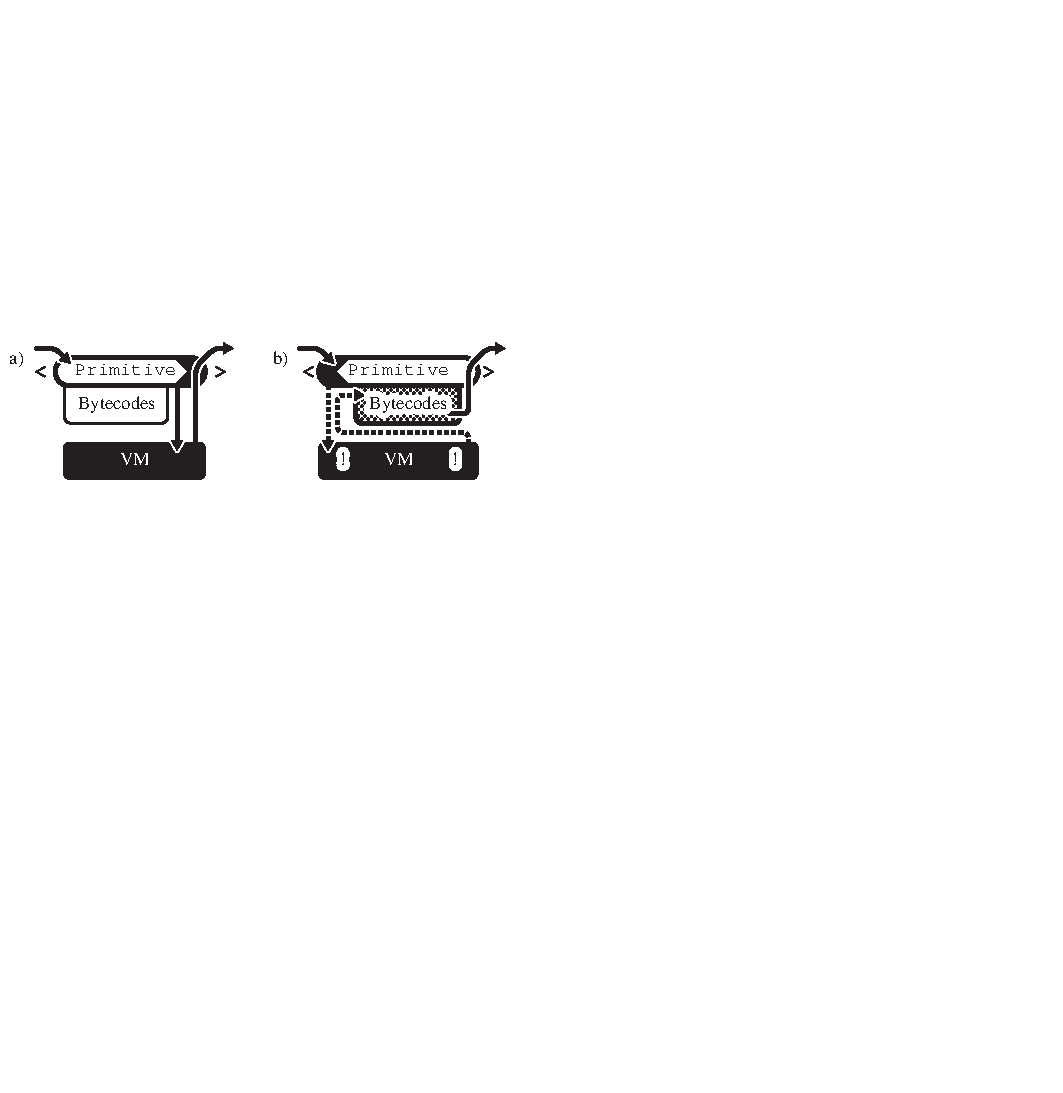
\includegraphics[scale=\imagescale]{smalltalkPrimitive}
	\caption[\PH Primitive]{Generic primitive methods in \PH: a) A primitive completely bypasses the bytecode, b) A failing primitive executes the bytecode as fallback.}
	\figlabel{benzo-smalltalkPrimitive}
\end{figure}

\noindent \B uses the primitives as a gate to enter the low-level world from the language-side.
Our custom primitive then executes the generated native code and returns to language-side. 
This code is appended inside the compiled method object.
When the primitive is activated, it  accesses the currently executed compiled method via a \VM function. 
\figref{benzo-nativeCodeMethod} shows the structure of a \PH compiled method that has native code attached to it.
We see the primitive tag on top, followed by the literal frame which holds references to symbols and classes used in the method.
The subsequent \PH bytecode is the fallback code executed only if the primitive fails. Only then appears the native instructions.
A marker at the end of the compiled method called trailer type is used to flag methods that actually have native code attached to them.
%
\begin{figure}[ht]
	\centering
	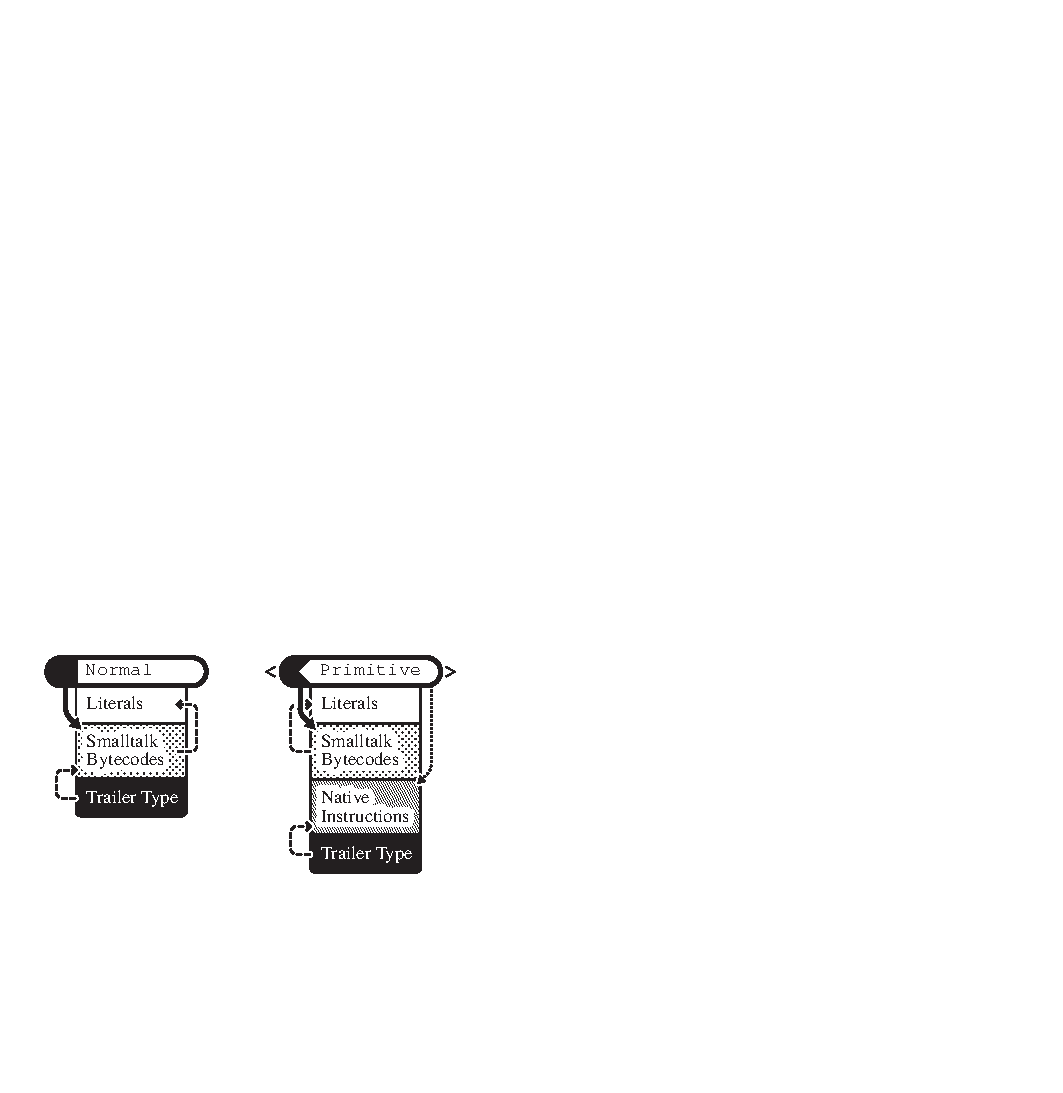
\includegraphics[scale=\imagescale]{nativeCodeMethod}
	\caption[\PH Compiled Method]{A standard \PH compiled method on the left and a method with appended native instructions generated by \B.}
	\figlabel{benzo-nativeCodeMethod}
\end{figure}

\noindent Since compiled methods are first-class objects it is possible to modify them at runtime and append the native code.
The primitive \ttt{primitiveNativeCall}, which is implemented by \B, is the responsible of running the native instructions in a \PH method.
The code example \ttt{interrupt3} shows a very basic application of our infrastructure.
\sm{Interrupt 3, really? That's the best name? You could also tell me that it is the standard interrupt for debuggers}
%
\begin{stcode}[label={lst:benzo-basic-native-code}, caption={\PH method using \B for very basic low-level debugging.}, escapeinside={@}{@}]{5}
interrupt3
	<primitive: 'primitiveNativeCall' 
	 module: 'Benzo' >
	Benzo generate: [ :asm | asm interrupt3 ]
\end{stcode}
%
The primitive named \ttt{primitiveNativeCall} on the first line tries to run the native instructions appended to the compiled method.
When there is no native code yet the primitive fails and on return it evaluate the rest of the \PH code in the method.
In \secref{benzo-language-side}, through more detailed examples, we describe how \B uses \PH code to generate the native instructions
\figref{nativeCodeMethodDetail} shows the resulting compiled method in full detail.
%
\begin{figure}[ht]
    \centering
    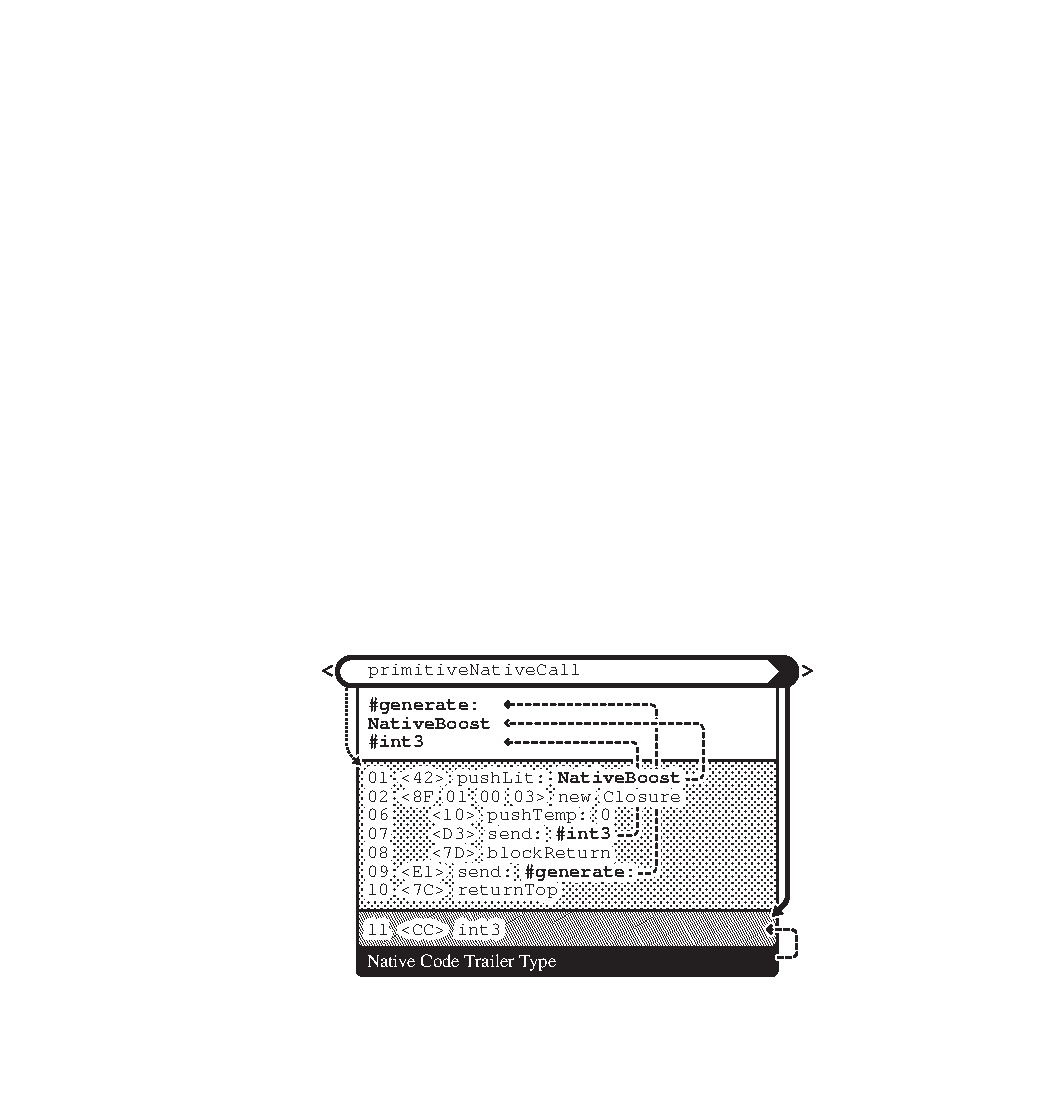
\includegraphics[scale=\imagescale]{nativeCodeMethodDetail}
    \caption[\ttt{CompiledMethod} With \B Code]{Example of \PH method with native code which calls the low-level debug exception handler \ttt{INT3}. The bytecode references objects indirectly via the literal frame residing at the beginning of the method.}
    \figlabel{nativeCodeMethodDetail}
\end{figure}

%----------------------------------------------------------------------------
\paragraph{Native Code Platform Interaction}
\seclabel{benzo-platform-interaction}

To ensure that the code is compatible with the current platform a \VM specific marker is expected at the beginning of the native code on the compiled method.
Upon activation \B compares this marker with the one from the current \VM.
If they do not match, \B signals a failure that causes the \VM to evaluate the fallback \PH code.
With this elegant approach \B regenerates native code lazily on new platforms.
Moreover, it does not have to flush the native code when the application is restarted on the same platform.
\sm{Reexecute vs. restart}

%----------------------------------------------------------------------------
\paragraph{Garbage Collector Interaction}
\seclabel{benzo-gc-interaction}
\seclabel{benzo-external-roots}

Compiled methods in \PH have a special section, the literal frame, which stores objects referenced in the bytecodes.
\sm{Did you introduce compiled methods as representing smalltalk methods? Because you use it in a way that's only unambiguous if you are a smalltalker}
Bytecodes then only have indirect access to these objects by indexing into the literal frame.
This simplifies the implementation of the garbage collector as it only has to scan the beginning of each method for possible references to objects. 
So the \GC only tracks \PH objects when they are in the method literal frame. 
The moving \GC of the \VM used for \PH has a significant impact on the low-level code we can generate using \B.
For instance it is not possible to statically refer to language-side objects from native code as object addresses change after each garbage collection.
Modifying the \GC to support regions of non-moving objects would solve this problem.
However, we chose to minimize the number of low-level \VM modification necessary to run our experiments and opted for a simpler solution.

\begin{figure}[ht]
	\centering
	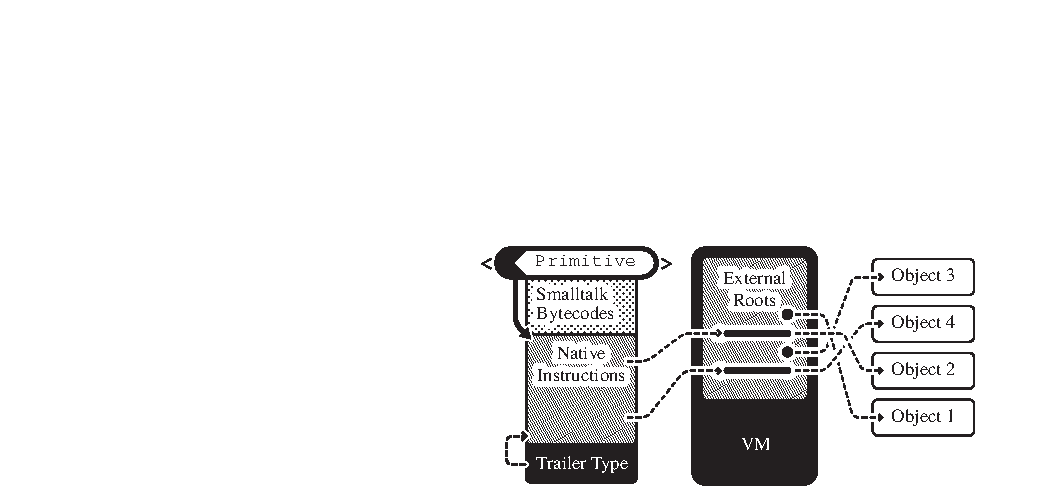
\includegraphics[scale=\imagescale]{externalRoots}
	\caption[Benzo External Roots]{Pointers to objects registered as external roots are pinpointed at fixed offset in global \VM-level object.
	\sm{You can argue differently here, GC depends on VM, (you are doing stuff that is supposed to be applicable in wider context) so, you are looking for a more general solution, one that doesn't put constraints on the type of GC... Voila, your laziness becomes something positive)}}
	\figlabel{benzo-externalRoots}
\end{figure}

\noindent \B accesses language-side objects through an indirection.
For indirectly accessing objects the \PH \VM already features a special structure, named \emph{external roots}.
This array has a fixed-location in memory which can be used to access moving language-side objects.
The \GC updates the addresses in this \VM structure after each run.
Hence we have the static address of the external roots object as an entry point to statically access \PH objects.
Summarizing, for accessing \PH objects within native code we first register it as an external root object and access it only indirectly.
This means that for native code, instead of a method-local literal array we share a global literal array as shown in \figref{benzo-externalRoots}. 
\B only adds an \ttt{Array} to the external root objects which is managed from language-side and administers all references.
\sm{Close to classic object table}

%----------------------------------------------------------------------------
\paragraph{\JIT Interaction}
\seclabel{benzo-jit-interaction}

When the \PH \VM starts the execution of dynamic generated code the execution environment changes slightly.
Similarly, when entering primitives or plugin code, the managed execution mode is left and a normal C-level execution environment is reestablished until the primitive finishes and the \VM jumps back to the jitted code.
These context switches impose an overhead and can be avoided in the case of calling native code.
For this reason we extend the \VM to support inlining of native code in the \JIT phase following the same strategy as other existing primitives which are inlined at \JIT-level.
%
\begin{figure}[ht]
	\centering
	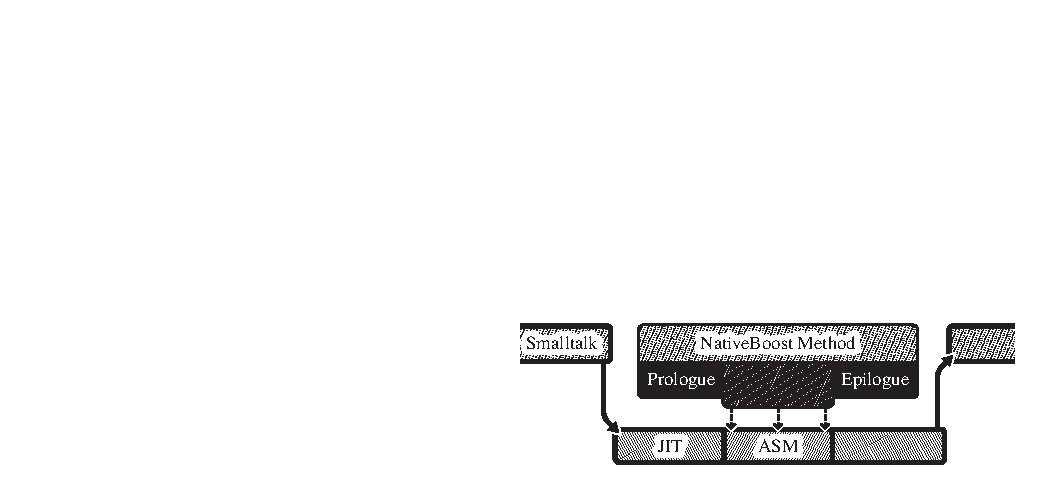
\includegraphics[scale=\imagescale]{nabujitoInline}
	\caption[\B \JIT Interaction]{\B inlining language-side native code into jitted mode.}
	\figlabel{benzo-nabujitoInline}
\end{figure}
%
\figref{benzo-nabujitoInline} shows how the native code from a \B enabled method is inlined into the \JIT infrastructure.
The \B prologue and epilogue used for managing the low-level stack are replaced by an adapted version for the \JIT.
The performance boost of this optimization is further discussed in \secref{benzo-issues-performance}.
\sm{Motivation first, why are you talking about this? Classic primitives have overhead, and you provide solution? Might not be novel,but in the context of your thesis goals it is necessary to achieve acceptable performance}


%----------------------------------------------------------------------------
\paragraph{Error Handling}
\seclabel{benzo-error-handling}

\B provides an error handling facility that allows one to return high-level error messages from the low-level code.
The native code builder provides a helper method called \ttt{failWithMessage:} that generates the proper assembler instructions to return a full error message. The following code shows an example application of this behavior.
\sm{Should you discuss the design of the native code builder? Is there anything relevant in there? I would expect it to be nicely designed to fit with your goals?}
%
\begin{stcode}[emph={asm}]{5}
failWithErrorMessage
	<primitive: 'primitiveNativeCall' 
	 module: 'Benzo' >
	 Benzo x86 generate: [ :asm :helper |
		helper failWithMessage: 'Value is not 0' ].
\end{stcode}
%
Under the hood, \B reuses the existing built-in error mechanism of \PH primitives.
However, primitives only allow for error number to be returned which limits the expressiveness of the error messages.
To circumvent this limitation \B assigns a unique error number for each error message pass to \ttt{failWithMessage:}.
\sm{It isn't a proper object that can be returned?
Shouldn't it be one in a nice clean design?}
The mapping between the two error message representation, its error number and the message string itself, happens at language-side.
\B simply reuses the existing infrastructure to improve the debugging tasks and promote a better interaction with developers.

%----------------------------------------------------------------------------
\subsection{\B's Language-Side Implementation}
\seclabel{benzo-language-side}
%----------------------------------------------------------------------------
As a key design decision, we determine to keep the interface to the low-level world minimal.
\sm{Goal!}
The following describes the features of \B at the high-level language-side.

%----------------------------------------------------------------------------
\paragraph{Code Generation}
\seclabel{benzo-code-generation}

\B delegates native code generation to a full assembler written in \PH. The following example shows how to use the assembler to generate the native code for moving \ttt{1} into the 32-bit register \ttt{EAX}.
%
\begin{stcode}{4}
Benzo x86 generate: [ :asm |
	asm mov: 1 asUImm to: asm registers EAX ].
\end{stcode}
%
The implementation first creates a slightly more abstract intermediate format.
The abstract operations can be extended by custom operations that may expand to several native instructions. 
\sm{Bottom up vs. top down discussion, in a thesis, I would expect top down,derived from goals and problems, I.e. By design, instead of an incidental solution that came to being without taking the overall goal into account. You need to tell me what you learned, not how you learned it/how you got to your solution}
The full features of the high-level environment are available when generating native code.
Hence complex instruction sequences can easily be delegated to other objects.
In the following example we use a \VM helper to instantiate an array. It is worth noting that all are standard message sends:
%
\begin{stcode}{5}
Benzo x86 generate: [ :asm :helper | | register |
	register := helper classArray.
	register := helper 
		instantiateClass: register
		indexableSize: 10
	asm mov: register to: asm resultRegister ].
\end{stcode}
%
\sm{Is that really high level? One thing here that's debatable is the API design, seems rather procedural. Instead of object oriented, the other thing, is is that really reflective or meta circular? How many places encode how an array is represented? The VM? Your library? Other things?

Superficially, it is just a code generation library that has nothing to do with the language it is implemented in, is that relevant? Do you need to defend such criticism? Or is that outside of the scope of your thesis?

That's why you need to get the problem statement very precise}
The \VM helper exposes a basic, low-level interface to access objects and its properties.
Additional methods cover the access to the external roots described in \secref{benzo-gc-interaction}.
In this case the \ttt{\#instantiateClass:\-in\-dex\-able\-Size:} will generate the proper native code to call to a \VM function and make sure that the side-effects of a possible \GC run are handled properly.
By default the value in the result register is returned back to the language-side. On \textsc{x86} this defaults to \ttt{EAX}.
In \secref{benzo-usecase} we introduce more substantial applications based on \B.

%----------------------------------------------------------------------------
\paragraph{Code Activation}
\seclabel{benzo-code-activation}
 
So far we only broadly described how \B activates the native code.
In a nutshell, we generate native code using our own language-side assembler and then we attach the native instructions to compiled methods as shown in figure \figref{nativeCodeMethodDetail}.
Additionally we mark the method to use a primitive defined \B plugin.
The \B primitive is responsible for the native code activation which consists of three main steps:
%
\begin{enumerate}[noitemsep]
	\item Check if there is native code in the actual compiled method and if it is compatible with the current platform.
	\item Generate native code if necessary.
	\item Activate the native code for execution.
\end{enumerate}

\noindent The first time a method with \B-based native code is activated the linked \B primitive will fail and run the normal \PH code in this method (see \secref{benzo-vm-interaction}).
This is where the actual native code generation happens.
As shown in previous examples, the native code is expressed in standard \PH code using our language-side assembler.
Once the whole code is generated, it is appended to the compiled method body leaving the existing \PH bytecodes intact.
Behind the scenes \B adds some more information to the code as the previously mentioned platform marker. 
After the native code is installed in the compiled method, we still run \PH code to restart the same \B-enabled method again.
%
\begin{figure}[ht]
	\centering
	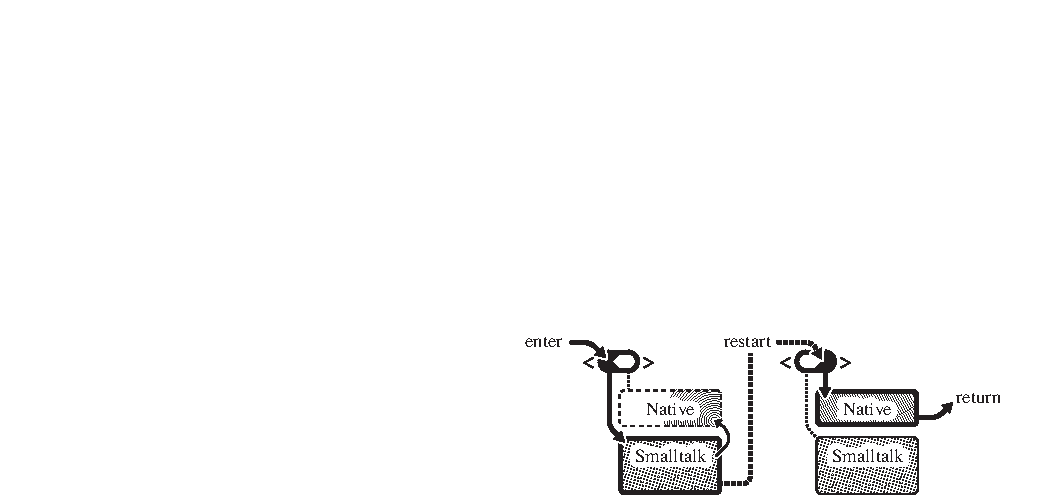
\includegraphics[scale=\imagescale]{nativeCodeActivation}
	\caption[\B Native Code Acivation]{Native code activation with \B: The first call triggers the code generation. Then the method is restarted and the native code executed.}
	\figlabel{benzo-nativeCodeActivation}
\end{figure}
%
For clarification we visualize the code activation process in \figref{benzo-nativeCodeActivation} and the following list describes the separates steps in more detail:
%
\begin{description}
\item[Activation:] In the first step (cf. \ding{182}) the \B primitive is activated.
	The primitive checks if the compiled method actually contains native code.
\item[Code Generation:] On the first activation there is no native code available yet.
	Hence the primitive will fail and the \PH body (cf. \ding{183}) of the \B-enabled method gets evaluated.
	This is where we use the \B \API and write native instructions as shown in previous examples.
\item[Code Installation:] After installing the native code in the method trailer, the \B-enabled method is reactivated with the original arguments (cf. \ding{184}).
	For activation \B uses \PH's  \ttt{\#perform:withArguments:} to reflectively restart the method.
\item[Method Reactivation:] Again we end up in the \B activation primitive (cf. \ding{185}).
	However, this time native code is present and thus the \B jumps to native code attached to the compiled method (cf. \ding{186} and returns the generated result.
\end{description}


% ===========================================================================
\section{\B in Practice}
\seclabel{benzo-usecase}
% ===========================================================================
In this section we present the outline 3 distinct solutions built on top of \B: A \FFI, dynamic primitives and a \JIT (\chapref{ffi} and \chapref{validation} provide more detailed insight).
Typically these implementations would require a custom-tailored \VM or specialized plugins.
However, we show that it is possible to implement them using the generic functionality provided by \B.

The chosen applications, starting with the \FFI, are increasingly more \VM bound.
Whereas the typical \FFI implementation is based on an separate plugin, dynamic primitives or a \JIT require persistent changes in the underlying \VM.


%----------------------------------------------------------------------------
\subsection{\NB: \B-based Foreign Function Interface}
\seclabel{benzo-ffi}
%----------------------------------------------------------------------------

\begin{figure}[h]
	\centering
	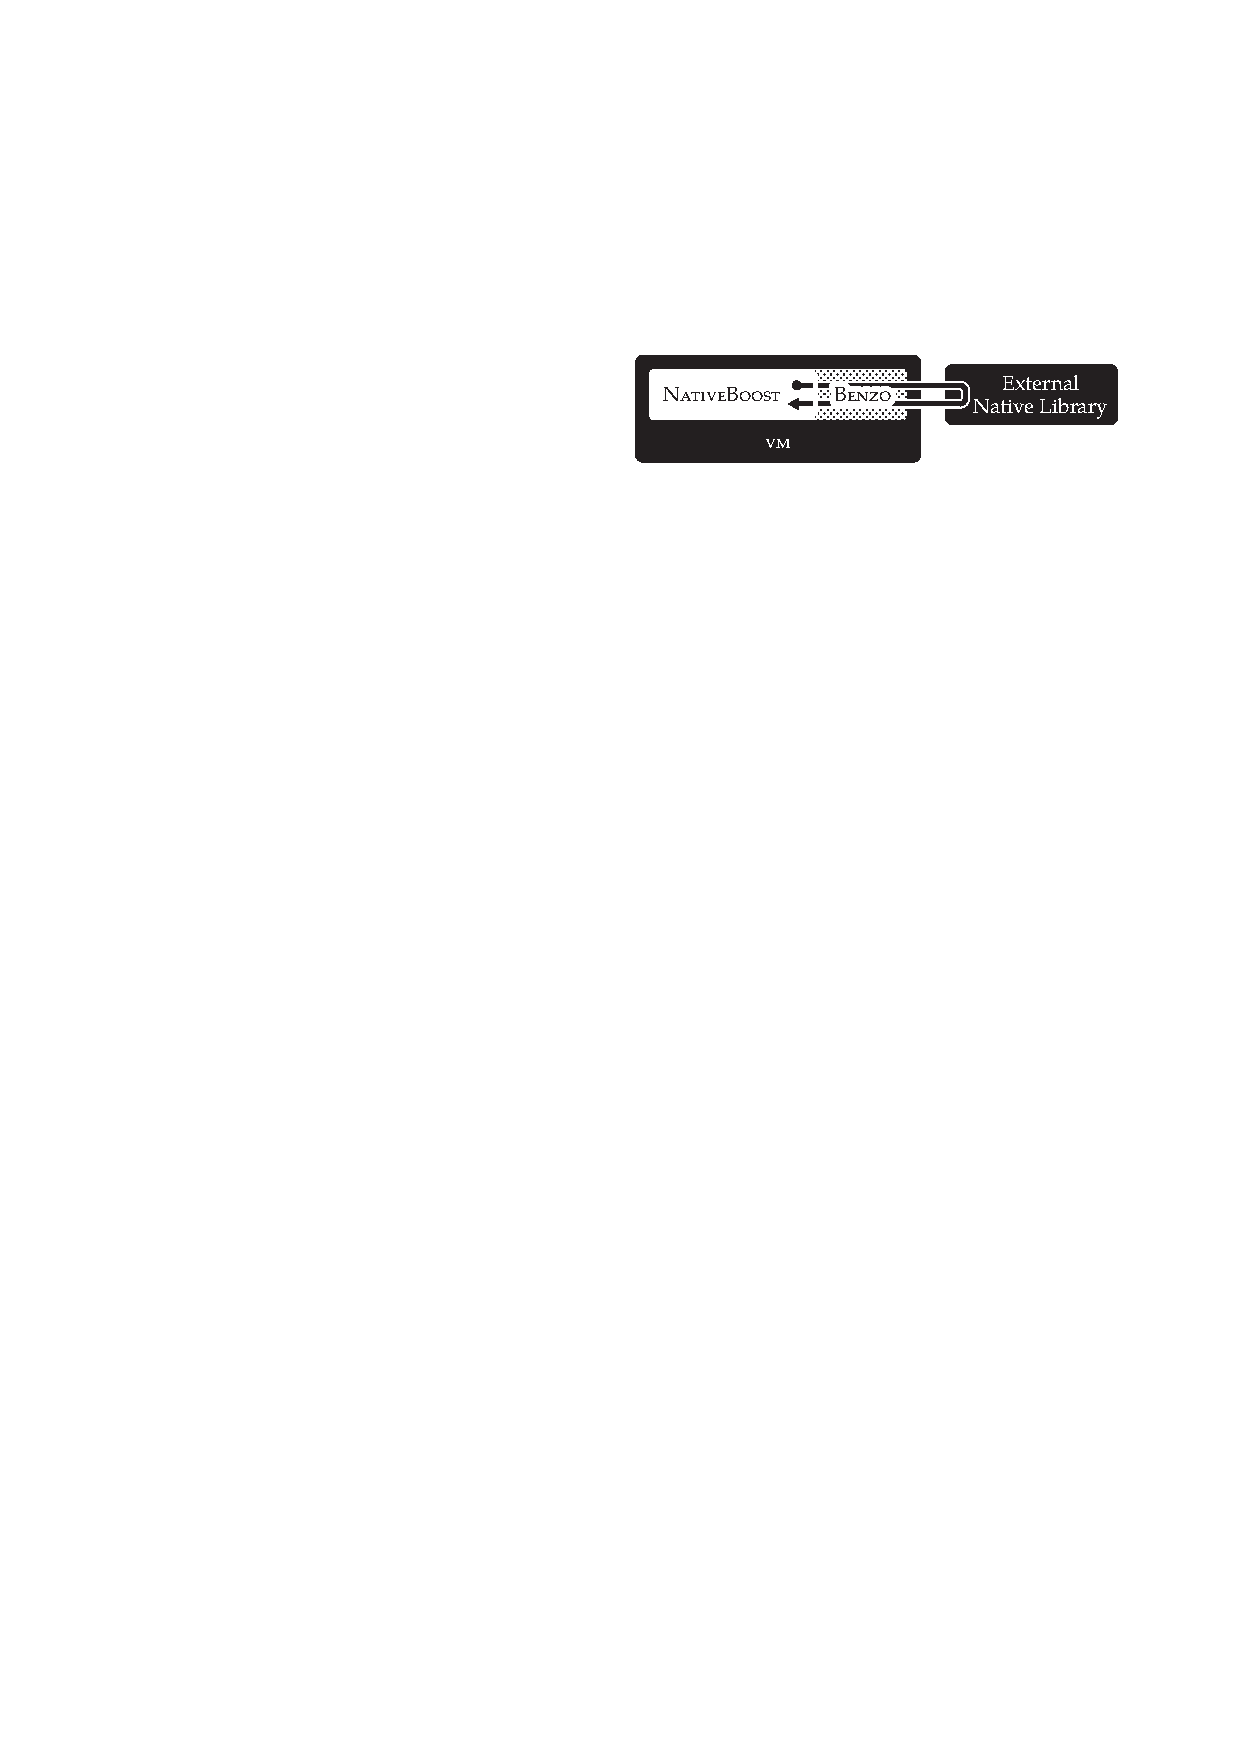
\includegraphics[scale=\imagescale]{nativeboost-overview}
	\caption[\NB Overview]{\NB generates native code at language-side with \B to perform an \FFI callout to an external function.}
	\figlabel{benzo-ffi-overview}
\end{figure}

\noindent \FFIs enable a programmer to call external functions without the need to implement additional \VM extensions.
\NB \cite{Brun13a} is a production-ready \FFI for \PH, developed on top of \B. 
For a detailed discussion of the implementation of \NB see \chapref{ffi}.
An \FFI implementation consists of two main parts: calling external functions and converting data between the two environments.
Typically a big percentage of these two parts are implemented at \VM-level with statically defined bindings.
Relying on \B's capability to dynamically generate and execute native code we developed a complete \FFI at language-side.
This way the \VM no longer requires to have a specific \FFI extension.

A very simple example to illustrate the functionality of \NB is to access the current environment variables with the \ttt{getenv} C function.
\ttt{getenv} takes a name as single argument and returns the value of that environment variable as a string:
%
\begin{stcode}{4}
getenv: name
    ^ NativeBoost call: 'String getenv(String name)'
\end{stcode}
%
In this example \NB automatically detects, using reflection, that the argument for the \PH method corresponds to the one of the low-level C function.
The most important aspect about this example is that it is written with standard \PH code, a property that extends to almost the complete implementation.
\NB, additionally to the native code activation, relies on two simple primitives provided by \B to retrieve addresses of external functions (\ttt{dlsym}) and to load external libraries (\ttt{dlopen}).

\NB generates the glue code to call external functions dynamically at run time.
It relies on \B's features presented in \secref{benzo-language-side} to generate and activate native code at runtime.
This gives \NB a significant advantage over static approaches: the generated native code is specific to the callout.
For instance in the \ttt{getenv} example, the marshalling code for converting from the internal \PH strings to C strings is written a small assembler routine.
In this specific context, the assembler code is faster than any language-side code.
Yet \NB is very flexible since all these conversion routines are defined at language-side. 
Each language-side library can define its own highly efficient conversion routines for types that are used in \FFI callouts, which is not directly possible to do with a \VM extension.


%----------------------------------------------------------------------------
\subsection{Reflective Primitives}
\seclabel{benzo-waterfall}
%----------------------------------------------------------------------------

\begin{figure}[h]
	\centering
	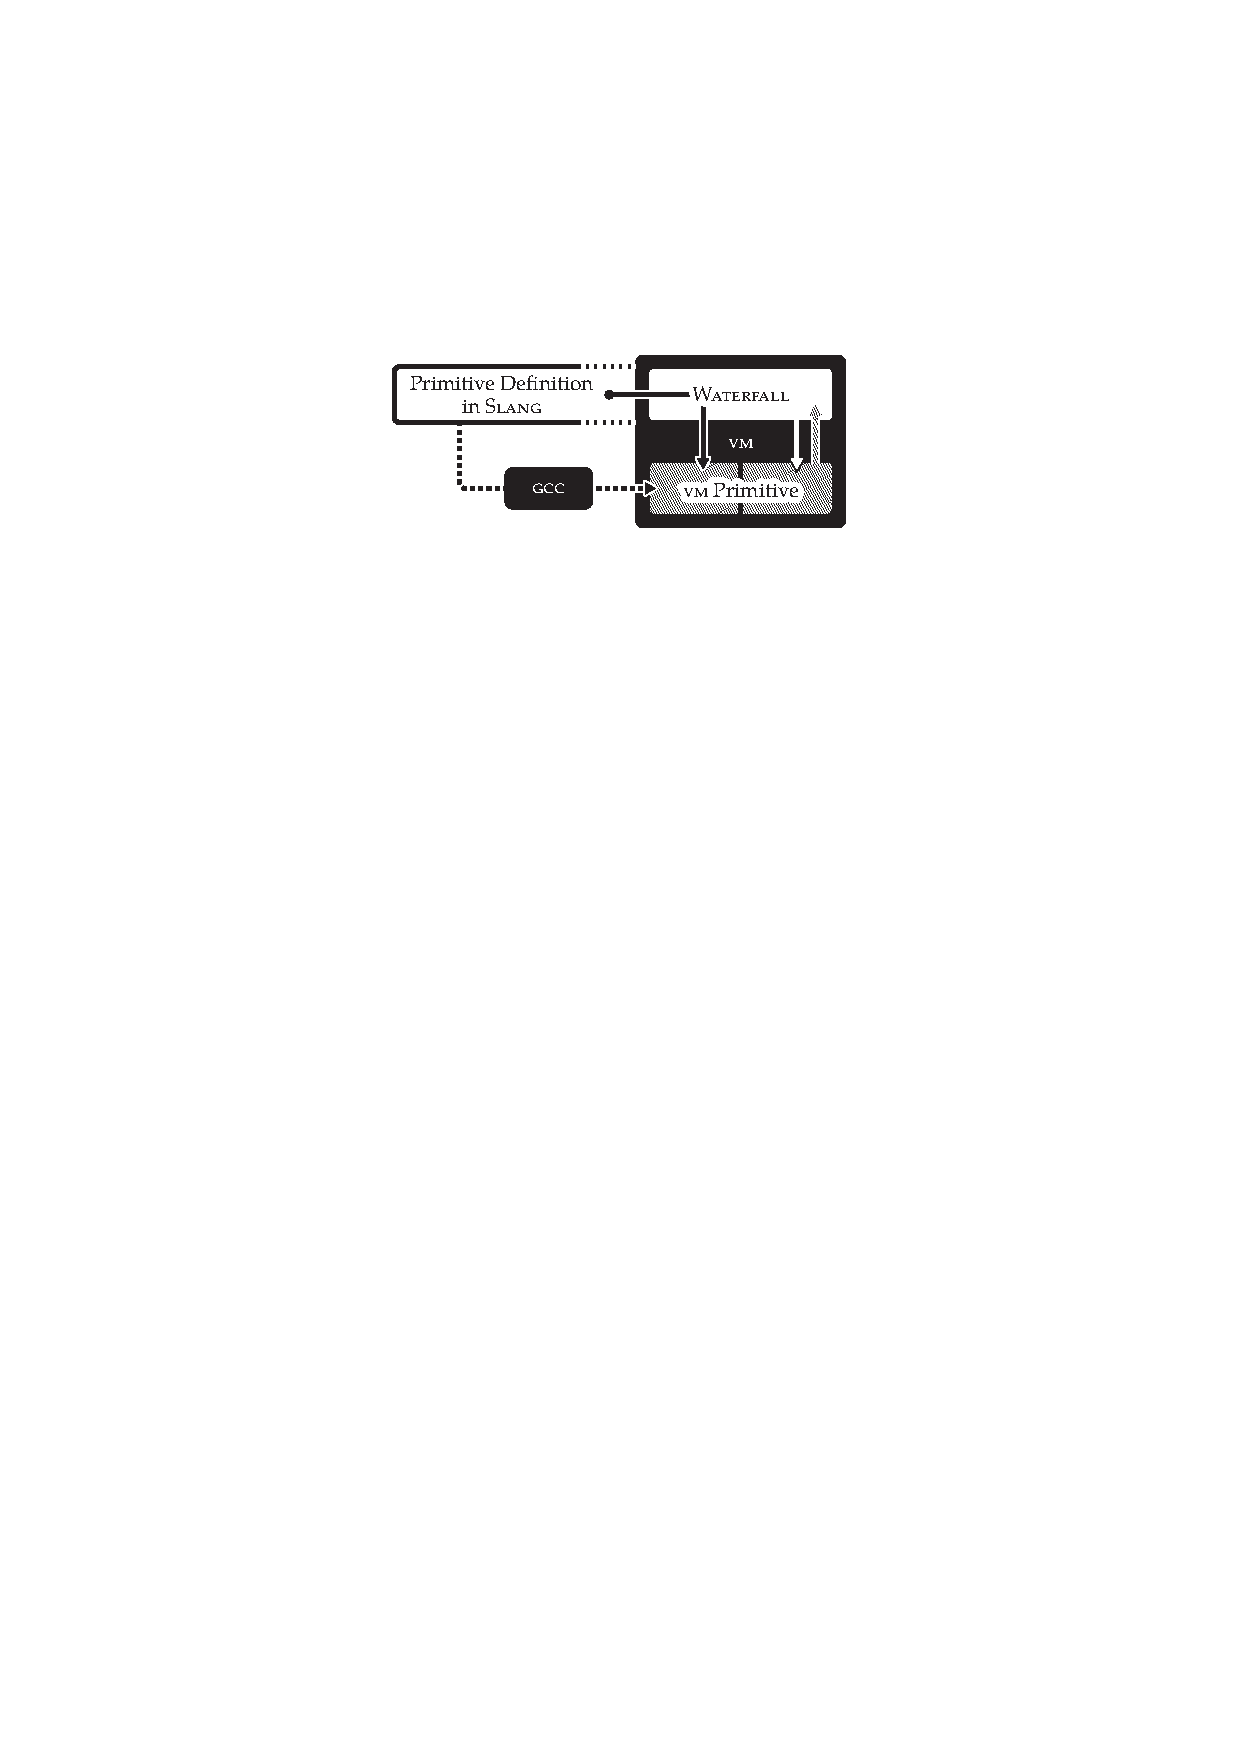
\includegraphics[scale=\imagescale]{waterfall-overview}
	\caption[\WF Overview]{\WF reuses the definitions of \VM primtives written in \Slang and compiles them dynamically. The same primitive definition is used for generating the static primitive at \VM compilation time.}
	\figlabel{benzo-waterfall-overview}
\end{figure}

\todo{by Guido Chari}
\noindent The second \B-based application we present takes the concept of our \FFI solution further.
\sm{Don't imply! Be explicit! The second is something... You neither name it nor give me clues what you are going to talk about.

And also, start out with telling my what waterfall is concretely, you are now telling me what it ain't, by telling me what native boost doesn't do. That can come later, first, I want to know why I should read this section}
\NB allows us to call external functions by generating the callout code at language-side.
From an abstract point of view we replace language-side methods with native routines.
\NB does not directly synthesize new features but only makes external functionality available to the language itself.

As explained previously in \secref{benzo-vm-interaction} \B uses \PH's primitives to activate native code.
Since \PH is an open system we can extend this behavior to existing methods.
Instead of simply adding new methods which call native code we present \WF, a solution that modifies existing primitive methods and replaces them with \B-based native code.
Instead of manually generating the sources for the primitives we reuse existing code.
The \VM used for \PH is metacircular, the \VM sources are written in the same language, in our case in a simplified subset of \PH called \Slang.
Hence, the complete definition of the \VM including the primitives can be made accessible at language-side by loading the \VM sources.
\WF then takes the primitive definition written in \Slang and compiles it to native-code.

As \figref{benzo-waterfall-overview} illustrates, \WF extends the lifetime of the metacircular \VM definition to the actual language runtime.
\sm{Why does this paragraph sound like it is going to talk about something very different? I first want to know how the compilation is done, do you have a slang interpreter or something?}
By default the primitive definitions written in \Slang are only used to generate the \VM source in an intermediate step.
A C-compiler such as \GCC generates the final binary.
By doing so the high-level primitive definitions are absorbed by the intermediate compiler infrastructure.
The final binary has no reflective capabilities anymore.
From within \PH we can only activate primitives but the abstract definition is no longer accessible.
Hence, we can not directly modify primitives directly without the original \VM sources loaded.
\sm{Are you sure you are fixing this, I.e., that the original code doesn't have to be present? Are you de compiling native code?

And, I still don't know how waterfall does the compilation, does it also use the c compiler?}

\WF provides a complete metacircular infrastructure for primitives.
\sm{Bla Bla, that doesn't tell me anything, because I don't know what that means in this context}
We use \WF to modify primitives on the fly.
For instance it becomes possible to instrument the crucial \ttt{basicNew} primitive, something that is almost impossible to achieve with pure language-side reflection.
\sm{I intercepted basicNew on the language side in my OMOP, no VM support necessary! I think you want to say something different.

(I did not change allocation, but I set the owner of each object by 'wrapping around' basicNew and basicNew:) }
Since this primitive is used for object creation, each attempt to monitor this primitive is doomed.
If the monitoring code itself would create a new object, infinite recursion would be inevitable.
\sm{True, but what's your point? Your solution ain't solving that either}
In \secref{val-waterfall} we explain in more detail the difficulty of such a task along with promising performance evaluations.



%----------------------------------------------------------------------------
\subsection{\NBJ \JIT Compiler Prototype Outline}
\seclabel{benzo-nabujito}
%----------------------------------------------------------------------------
\todo{Adapt to the findings of \NBJ that it is currently not possible to implement on top of the \VM}
In this section we present \NBJ, a \B-based approach for a language-side \JIT compiler.
\NBJ goes even further than \WF using almost the same techniques.
\sm{I still have not even an intuition what waterfall does :(}
However, instead of focusing on primitives, \NBJ generates native executable code for standard \PH methods.
Primitives tend to be more low-level, whereas \NBJ focuses on high-level \PH code. 

\begin{figure}[h]
	\centering
	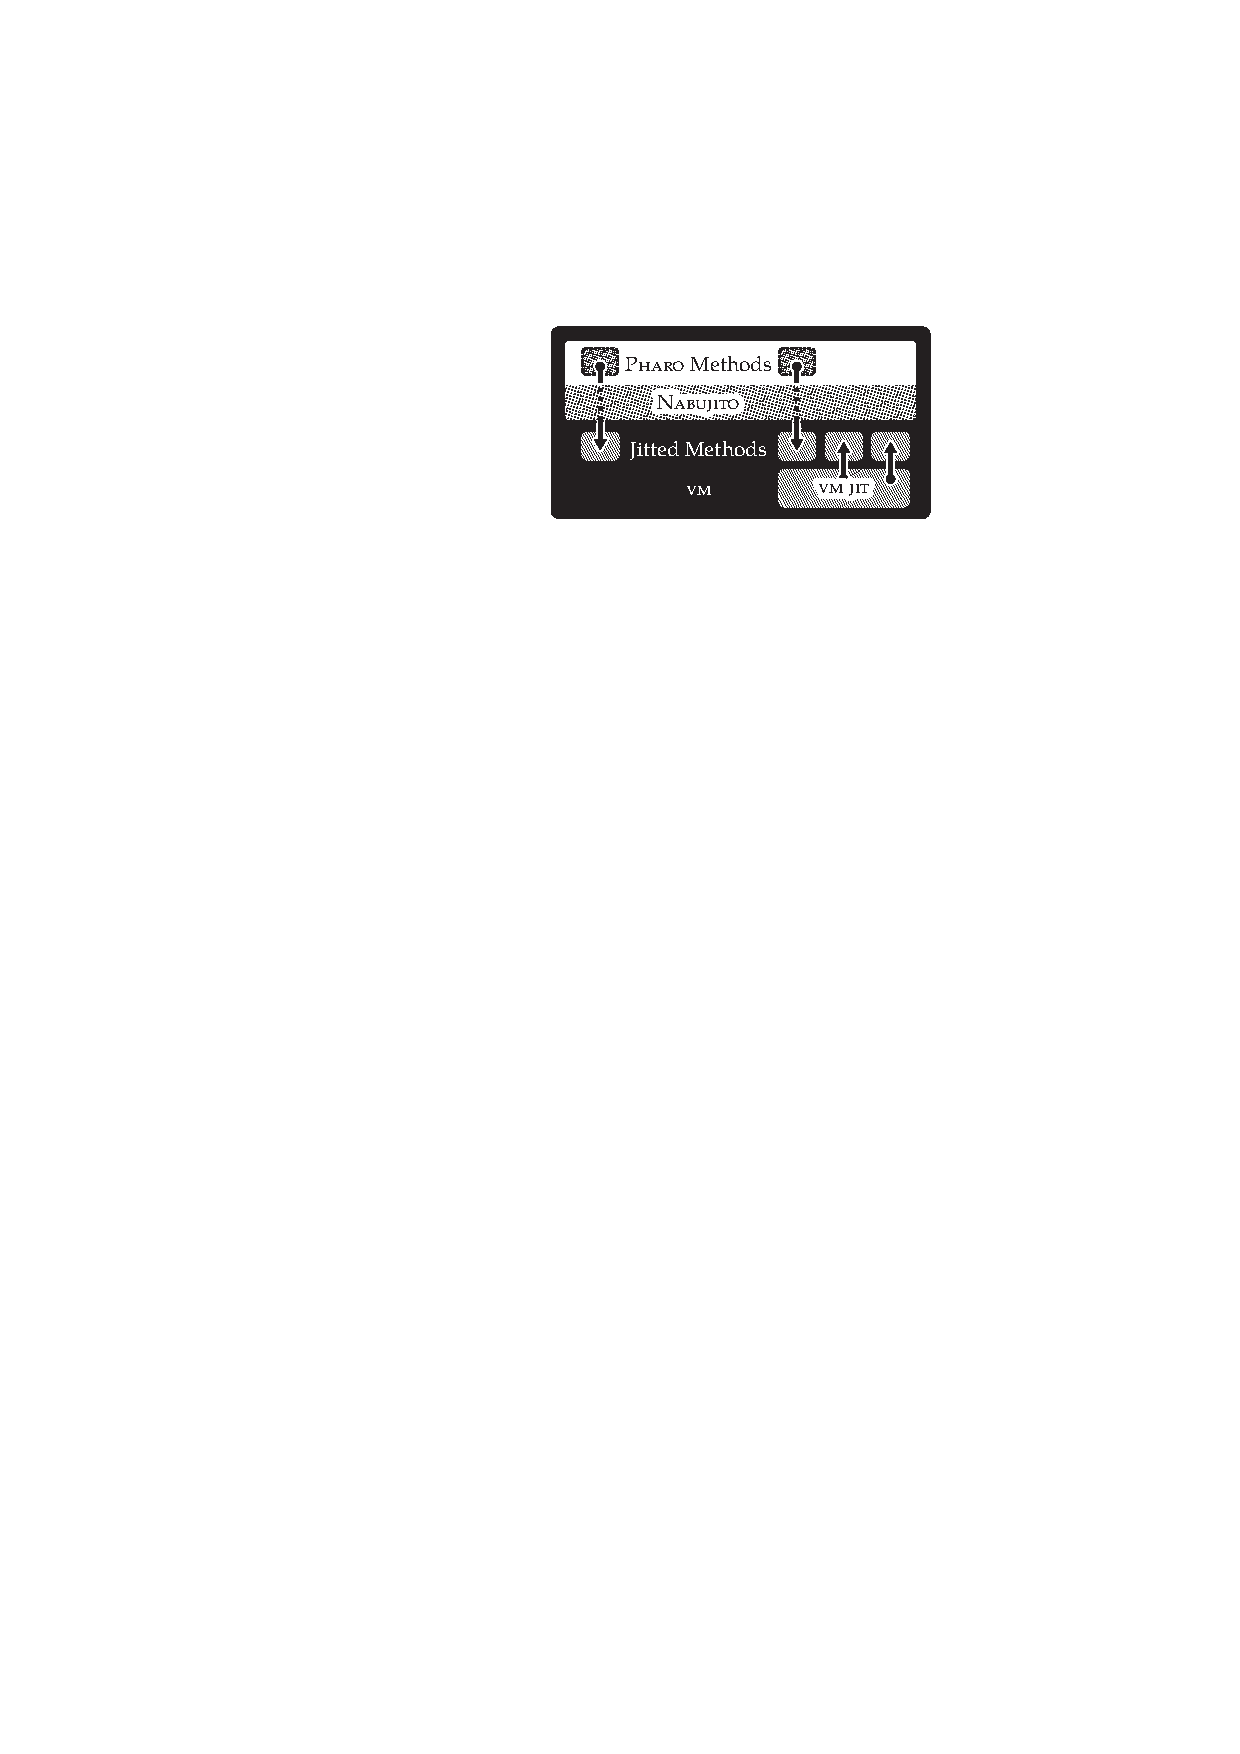
\includegraphics[scale=\imagescale]{nabujito-overview}
	\caption[\NBJ Overview]{\NBJ compiles standard \PH methods with the help of \B to the same format the \VM \JIT uses.}
	\figlabel{benzo-nabujito-overview}
\end{figure}

\noindent The \PH \VM (originally \urlfootnote{\textsc{Cog vm}}{http://www.mirandabanda.org/cog/}) already comes with a \JIT that translates bytecodes to native instructions.
It transforms \PH methods into slightly optimized native code at runtime.
The most complex logic of the \JIT infrastructure deals with the dynamic nature of the \PH environment.
Methods and classes can be changed at runtime and that has to be addressed by the \JIT infrastructure.
This implies that an efficient \JIT infrastructure needs substantial access to language-side structures; in our case classes, methods.
\sm{Really? I don't believe that. That only means you need to be able to invalidate code, something that ever speculative \JIT does, and you said before that there aren't any VMs fulfilling your criteria. So, be more precise here, this is too sloppy and too broad of a statement}
This information is readily accessible in \PH through the standard reflective \API.
However, at \VM-level this requires more effort, and thus imposes strong requirements on the design of classes and methods at language-side.
The \JIT infrastructure is a hybrid between \VM logic and language-side reflection.

The \JIT compiler, by which we refer in this context to the transformation of bytecodes to native code, represents a small part of the whole \JIT infrastructure.
There exists more important stages \sm{Reference unclear, what is more important than what?} as an additional register allocation pass to reduce the number of stack operations \cite{Mira99a,Mira11a}.
The existing \JIT infrastructure is implemented in \Slang \cite[Ch.\ 5]{Blac09a} as the rest of the \VM.
We believe that a hard-coded static and low-level implementation is not optimal for several reasons:

\begin{itemize}
	\item Optimizing \PH code requires strong interactions with the dynamic environment.
	\sm{Why? Java proves you wrong by your own criteria, I believe, as does Self most probably}
	
	\item Accessing language-side properties from the \VM-side is hard.
	\sm{Hard? Or impossible? And why is that? Just because the interface isn't well defined?
	This criterion is not useful as it is phrased now}
	
	\item Changing the \JIT compiler requires changes at \VM-level.
	\sm{So what? You are implying here assumptions about development approach, stuff you discussed earlier, I think. So, changing the VM takes a lot of effort, which you outlined earlier? That's your point? You want that to be possible much more interactively? Then say that, instead of broad phrases}
	
	\item The \JIT reimplements primitives for optimization reasons resulting in code duplication.
	\sm{This problem is now noted down on the list of things your reviewers are expecting you to solve, I hope you do...}
\end{itemize}

\paragraph{Implementing \NBJ with \B}
Motivated by the aforementioned implications of a \VM-level \JIT we conceived \NBJ a prototype \JIT compiler based on \B.
\NBJ is an experimental \JIT implementation which replaces the bytecode to native code translation of the existing \JIT infrastructure with a dynamic language-side implementation.
\NBJ is implemented as a visitor over the existing intermediate bytecode representation. 
Additionally we reimplemented \sm{Oh oh, didn't you say reimplementing stuff is evil? Perhaps make this more clear, and avoid the word, you just put on the list of things you want to solve...} vital native routines for the \JIT which are not directly exported by the \VM using \B. 
\NBJ relies on the following \VM-level infrastructure to manage and run native code for any \PH method:

\begin{itemize}[noitemsep]
	\item Fixed native code memory segments.
	\item Routines for switching execution contexts.
	\item Native stack management.
\end{itemize}

\paragraph{Dynamic Code Generation}
For standard methods \Nabujito takes the bytecodes and transforms them to native code.
It also applies optimizations such as creating low-level branches for \PH level branching operations like \ttt{if\-True:}.
Optimizations for additional methods are all implemented flexibly at language-side.
Wherever possible, we reimplement the same behavior as the existing native \JIT compiler.
Eventually the native code is ready and \B attaches it to the existing compiled method.
When the language-side jitted code is activated \B ensures that we do not have to leave the \JIT execution mode, and thus we can call methods at the same speed as the existing \JIT.
\secref{val-nabujito} gives a more detailed insight of the design and performance of \NBJ.



%============================================================================
\section{Performance}
\seclabel{benzo-issues-performance}
\seclabel{benzo-performance}
%============================================================================

In this section we discuss the general performance characteristics of \B for the three example applications outlined in the previous section.
A more detailed validation is presented later in \secref{ffi-performance} (\FFI), \secref{val-waterfall-performance} (\WF) and \secref{val-nabujito-performance} respectively.

\paragraph{One-time Code Generation Overhead} 
\B allows the generation of specialized and thus efficient native code.
In \secref{benzo-benzo} we explained how \B causes only a one-time overhead for native code generation. 
Thereafter it is cached for later activations.
The three use case presented in \secref{benzo-usecase} heavily benefit from this fact.
Generating code at language-side poses a significant overhead compared to invoking a precompiled native implementation.
However, this is only a one time overhead.
For instance the \B-based \FFI implementation presented in \secref{benzo-ffi} outperforms a \VM-level \FFI-plugin due to a more flexible language-side implementation which generates specialized code for each \FFI callout. 
These results are shown in the following \tabref{benzo-ffi-performance-simple}.

% ---------------------------------------------------------------------------
\subsection{\B-based \FFI}
\seclabel{benzo-nb-performance}
% ---------------------------------------------------------------------------

The first mini performance evaluation we present is for \NB the \B-based \FFI.
Compared to a static plugin-based \FFI implementation \NB has only a one-time startup overhead.
Generating the native code at language-side is substantially slower than directly setting up all the conversions and calling the external functions from C code. 
In certain cases the penalty for the language-side code generation of \NB is as high as a factor of 100 compared to classic approaches.
\sm{Approaches, to what do you compare exactly? Be more precise with those comparisons, you are slower than what exactly? Otherwise, I stop reading, because you are just saying the your whole approach is doomed...}
Under the assumption that the method is called several times this overhead may be considered negligible.
An in-depth evaluation of \NB comparing against other solutions is presented later in \chapref{ffi}.
The following table contains a performance comparison of three different \FFI implementations for \PH that represents the typical showcase.
\sm{Use case, not show case, showcase is something specifically selected that shines, nothing typical about that}

\begin{table}[!ht]
    \centering
    \begin{tabular}{rSS}
                   					& {Call Time [ms]} & {Relative Time} \\\midrule
        \NB         				& 10.53(35)        &        1.0 \\
        \Alien, language-side \FFI  & 31.09(94)        & \approx3.0 \\
        C-\FFI, plugin-based \FFI   &  9.55(64)        & \approx0.9
    \end{tabular}
    \caption[Basic \B-based \FFI Performance]{Different \FFI implementations in \PH evaluating \ttt{abs(int)}. \Alien does marshalling at language-side while \FFI does everything in \VM plugin written in C.}
    \tablabel{benzo-ffi-performance-simple}
\end{table}

\noindent \tabref{benzo-ffi-performance-simple} measures the accumulative time of 100'000 \FFI calls.
Included in these numbers is at least one additional \PH message send to activate the \NB method containing the actual call to the C function.
\NB outperforms the existing language-side \FFI (\Alien) and the implementation (C-\FFI).

The existing language-side \FFI has a generic plugin to call C-functions and performs type-conversions at language-side.
However, converting \PH objects from and into low-level data is comparably expensive.
In \NB this happens directly in custom generated native code and is thus significantly faster.
The plugin-based \FFI is also slower than \NB since it still has generic conversion function for \PH objects, albeit written in C and thus faster than in \Alien.
However, \NB custom tailored \ASM code is still faster than the hard-coded C counterpart.
\sm{There something wrong with either the number so the text, the CFFI is faster according to call time}

This simple \FFI evaluation already highlights the core benefit of \B to generate very customized native code when needed.
Yet we have to emphasize that \NB is based on the \B infrastructure whereas the other solutions require both a \VM plugin whose sole purpose is to enable the \FFI functionality.
Furthermore \NB benefits from the \JIT interaction described in \secref{benzo-jit-interaction}.
This optimization is especially an important optimization factor when calling out small helper routines where the context switch from jitted mode is no longer negligible.

% ---------------------------------------------------------------------------
\subsection{\B-based Dynamic Primitives}
\seclabel{benzo-wf-performance}
% ---------------------------------------------------------------------------

As the second performance evaluation of \B we present a simple use case of dynamically implementing a primitive with \WF.
For comparing performance we implement a very simple integer operation primitive (\ttt{$>$}) using three different approaches.
The first approach is the implementation with \WF.
The second is to run the language-side implementation that is triggered whenever the standard primitive failed.
Finally the fast standard primitive provided by the \VM.
We run the three approaches by measuring the cumulative time over one million primitive activations averaged over 100 runs.
The absolute numbers are less important than the relative factor between them.
We present the results of this experiment in \tabref{benzo-waterfall-performance}.
%
\begin{table}[!ht]
    \centering
    \begin{tabular}{rSS}
		Primitive Type  & {Running Time [ms]} & {Relative Time} \\\midrule
		\VM			    &   6.40(14)          &         1.0 \\
		\WF             &  22.80(17)          & \approx 3.6 \\
        Reflective	    & 195.00(16)          & \approx30.0
    \end{tabular}
    \caption[Basic \B-based Dynamic Primitive Performance]{Comparing running time of different implementations of integer arithmetic primitive.
    \sm{While it might not matter for the numbers, for a clear setup it would be advisable to not include the failing of the primitive in the measurement.
    
    From the text it is not clear whether you do or don't }}
    \tablabel{benzo-waterfall-performance}
\end{table}
%
\WF clearly outperforms a purely reflective solution.
As explained in \secref{benzo-waterfall}, replacing a crucial primitive with simple language-side is not straight forward.
If the replacement code triggers the very same primitive again we are trapped in a meta-recursion loop \cite{Chib96a}.
To avoid this, the \PH code for the replacement of \ttt{$>$} checks that the current activation of the primitive is not recursive.
This comes at a substantial cost and is the main overhead factor.

\WF is a factor $3.6$ slower than the standard implementation.
First we have to state that \WF uses a very simplistic compilation strategy with many optimizations opportunities left out.
Second, the optimized \VM primitive is also reimplemented in the \JIT to avoid the overhead of switching execution context (see \secref{benzo-vm-interaction}).
\sm{I don't get the second part}

This results thus makes a whole new set of runtime extensions feasible that were previously limited by their strong performance penalty.
Furthermore the performance penalty over a completely optimized \VM solution that has extreme optimization techniques, such as inlining and register allocation, is less than a factor of $4$.
A more detailed analysis of \WF is available later in \secref{val-waterfall-performance}.
\sm{If you do detailed stuff later, I would drop this 'mini' stuff here. One evaluation is enough, this section/chapter can stand on its own and should make the ideas clear}


% ===========================================================================
\section{Extending the Language Runtime}
\seclabel{benzo-related}
% ===========================================================================
\todo{try to push to background chapter}
In the context of \B we see a variety of related work spawning different abstraction levels.
On a more abstract scale \B allows for a new way of extending the complete language runtime, hence we classify the related work according the following categories show in \figref{benzo-extensionComparison}: general language-side extensions, extensions using reflection, \VM-level extensions, and hybrid approaches.

We present now an overview of the approaches used to extend a language runtime and expose their limits.
High-level languages are in general sustained by a \VM and a vast set of libraries written in the language itself. 
Extending or improving the existing language runtimes is a difficult task.
In most cases the \VM is considered as a black box.
Additionally the \VM is written in a completely different language using another abstraction level than the one it supports.
Typically high-level language \VMs are written in C or C++.
To address extensions in this context there exist some known approaches:
\sm{All the introduction stuff should be done in the proper chapter, 2, I guess }

\begin{description}[noitemsep]
	\item[Language-side Library] based on implementing a new or existing library. 
	\item[Reflective Extension] relying on reflective features of the language. 
	\item[\VM Extension] by writing plugins or changing the core of the \VM.
	\item[Hybrid Extension] by accessing external libraries using \FFI.  
\end{description}
%
The relation between the side concerning the abstraction and implementation levels (\VM vs. language) of these extensions is illustrated in \figref{benzo-extensionComparison}.

\begin{figure}[h]
	\centering
	\begin{subfigure}[t]{0.45\textwidth}
		\centering
		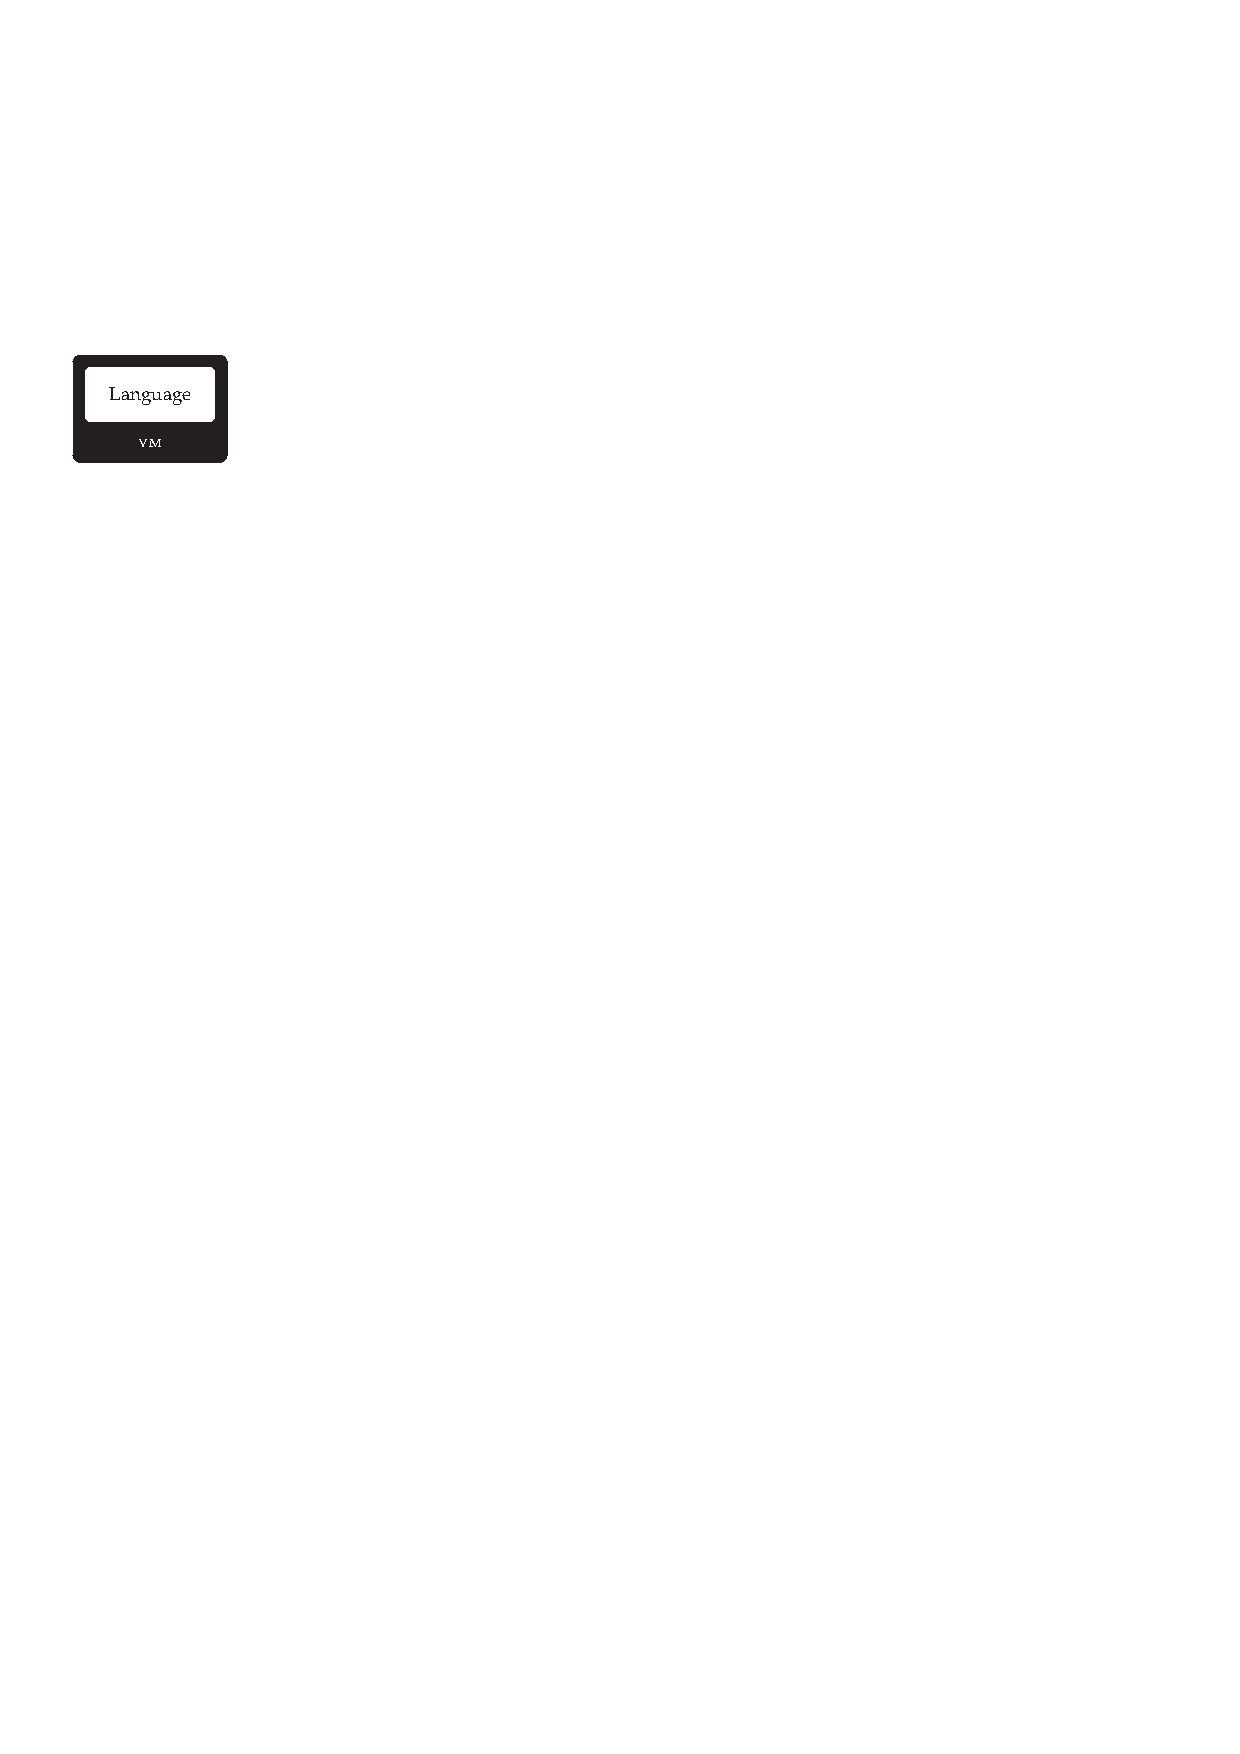
\includegraphics[scale=\imagescale]{extension-language}
		\caption{Language running on a standard, unmodified \VM.}
	\end{subfigure}\hspace{0.09\textwidth}
	\begin{subfigure}[t]{0.45\textwidth}
		\centering
		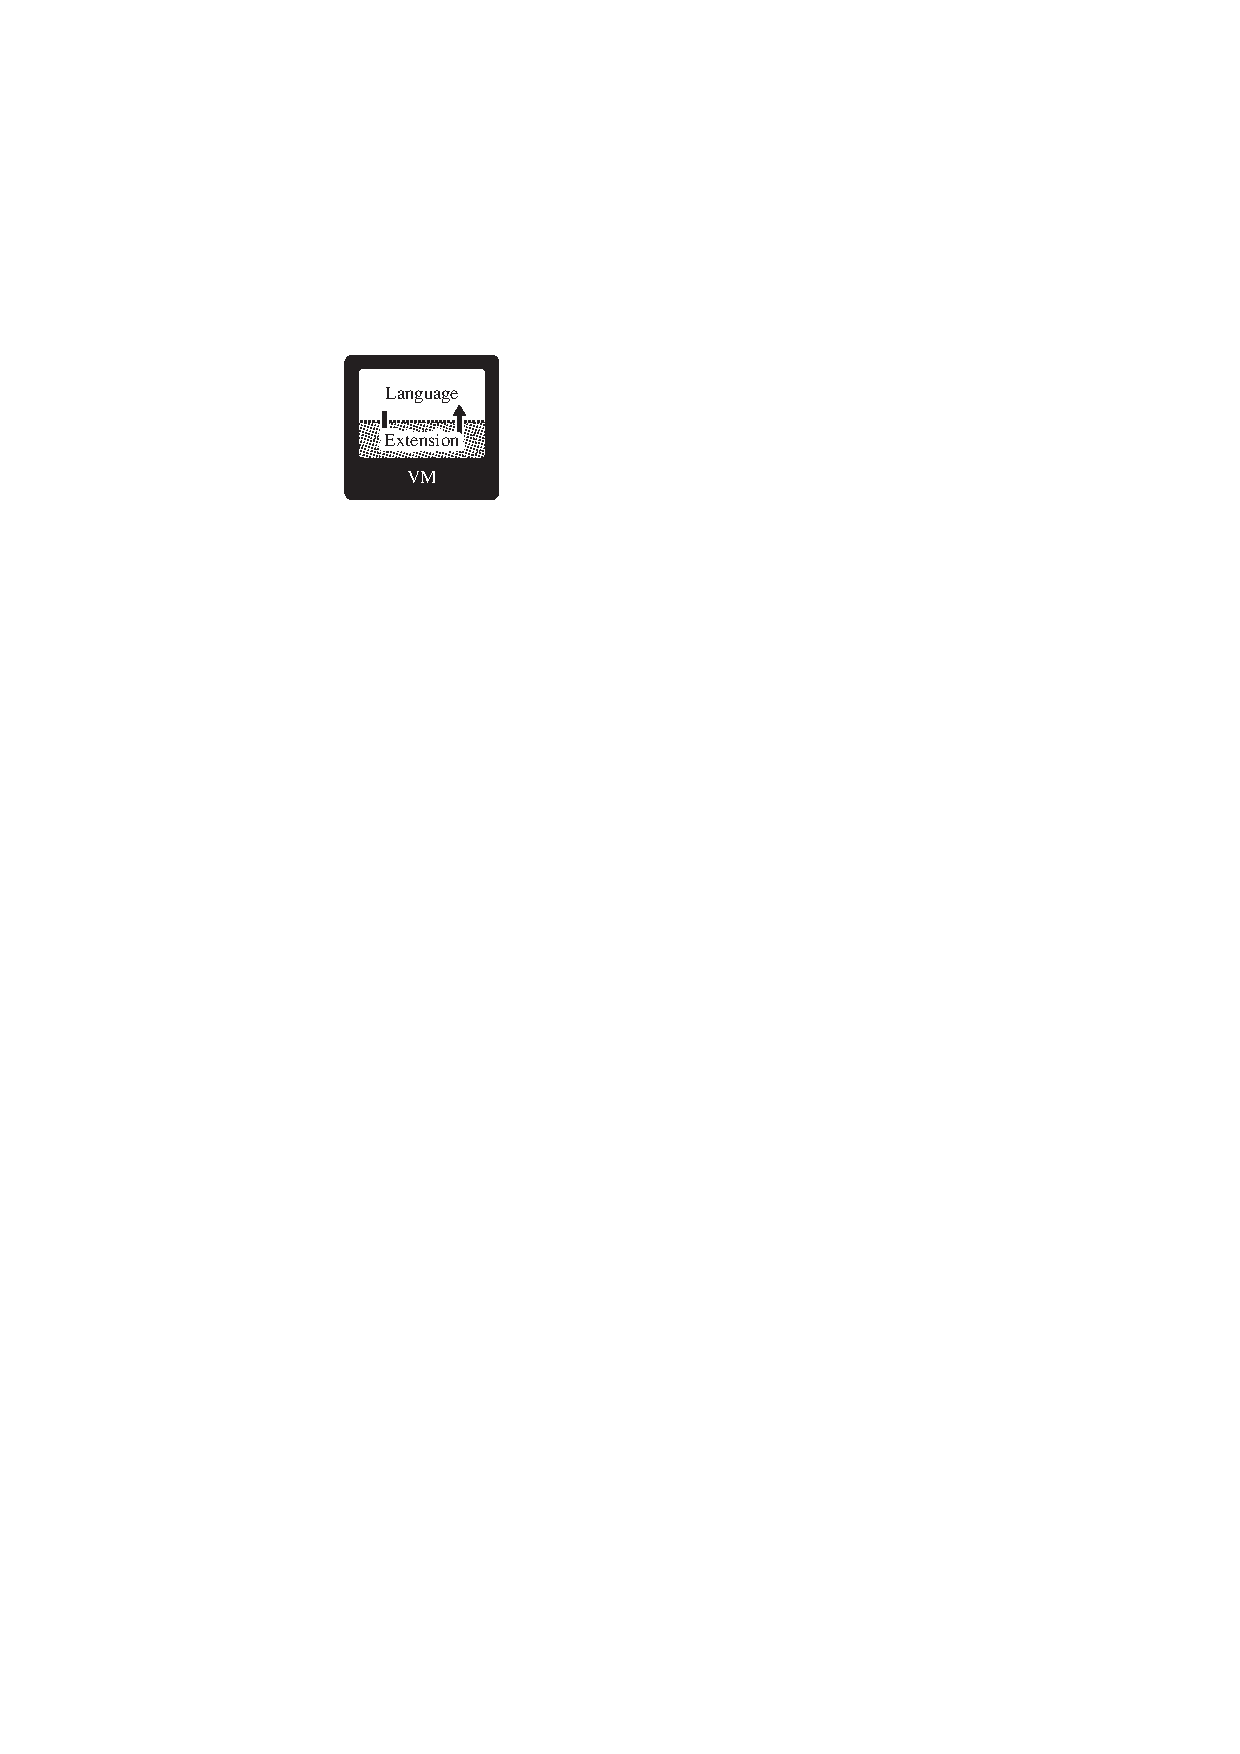
\includegraphics[scale=\imagescale]{extension-language-library}
		\caption{Language-side implementation of an extension.}
	\end{subfigure} \\
	\vspace{\baselineskip}
	\begin{subfigure}[b]{0.45\textwidth}
		\centering
		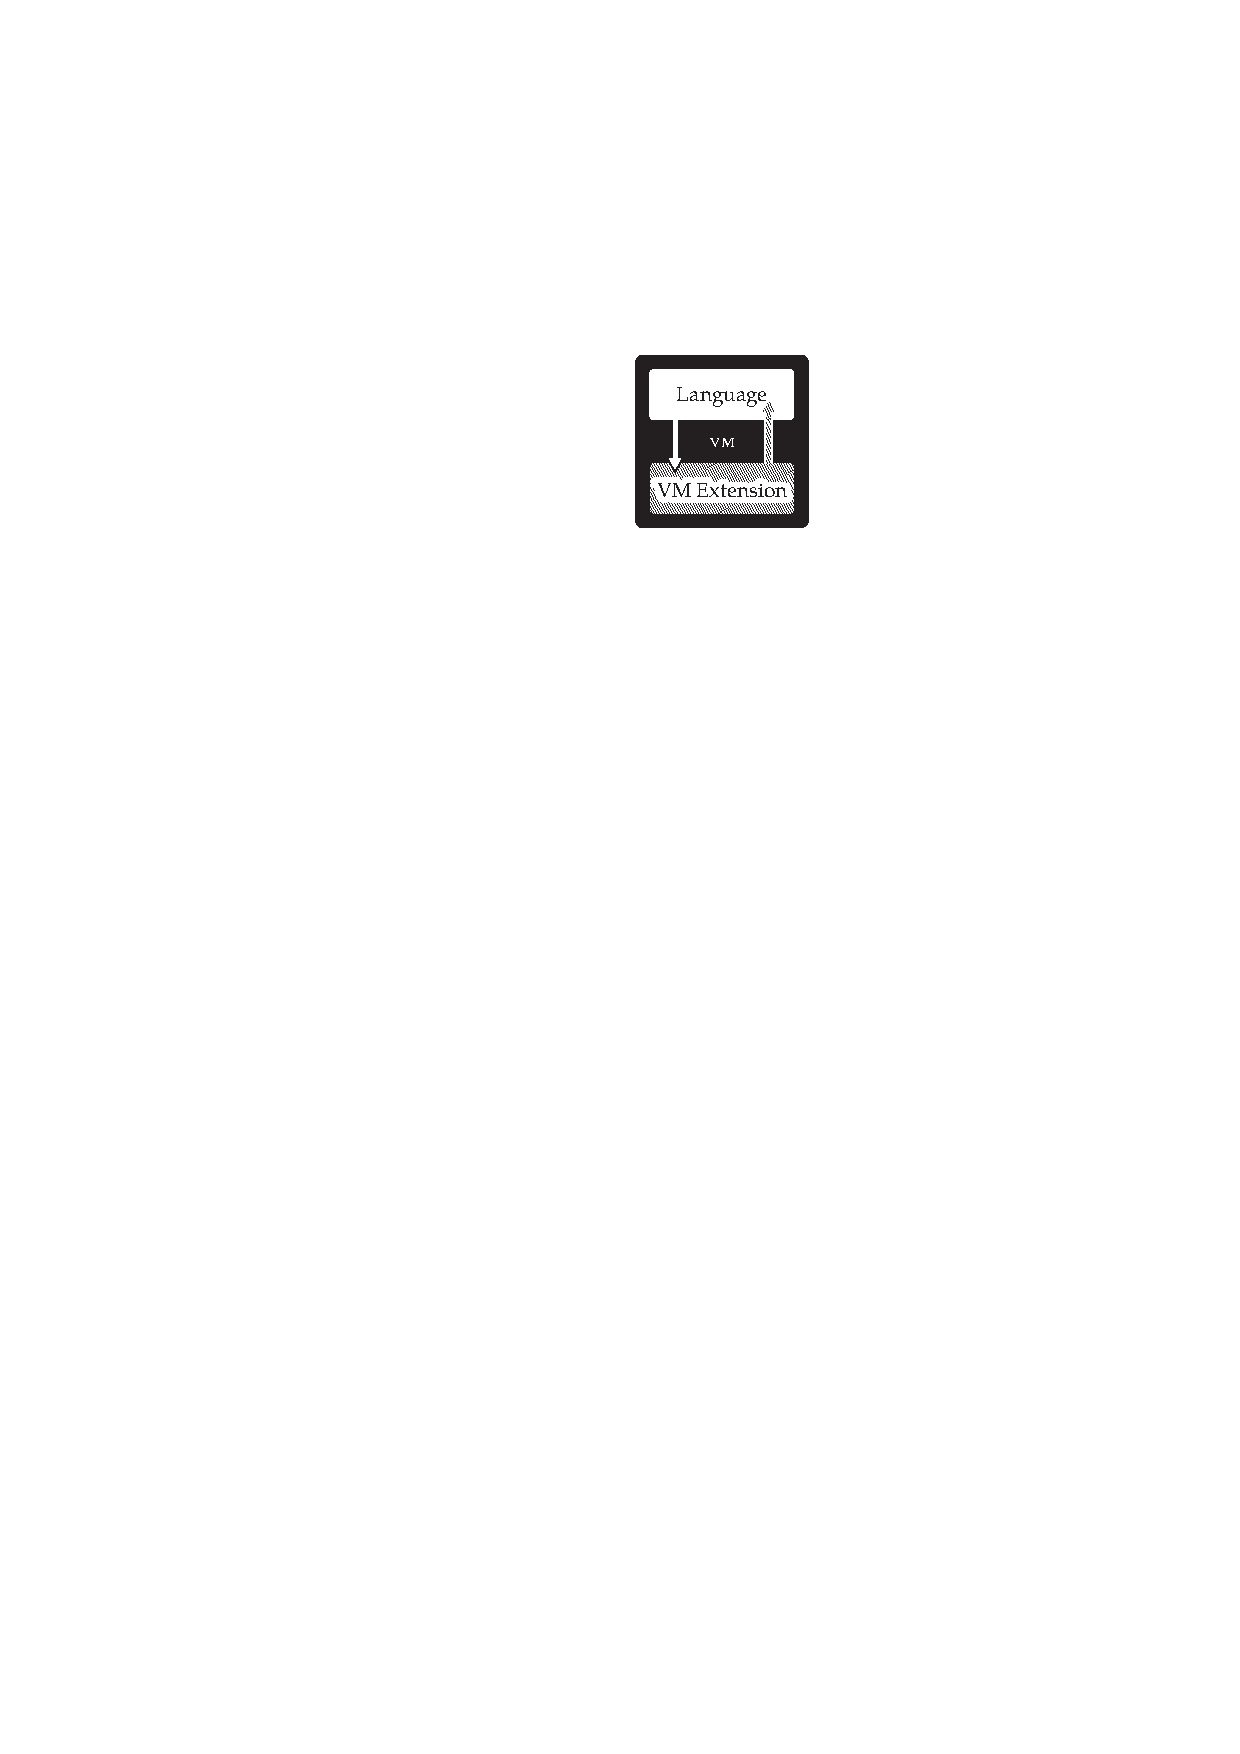
\includegraphics[scale=\imagescale]{extension-vm}
		\caption{Language using features from a \VM extension.}
	\end{subfigure}\hspace{0.09\textwidth}
	\begin{subfigure}[b]{0.45\textwidth}
		\centering
		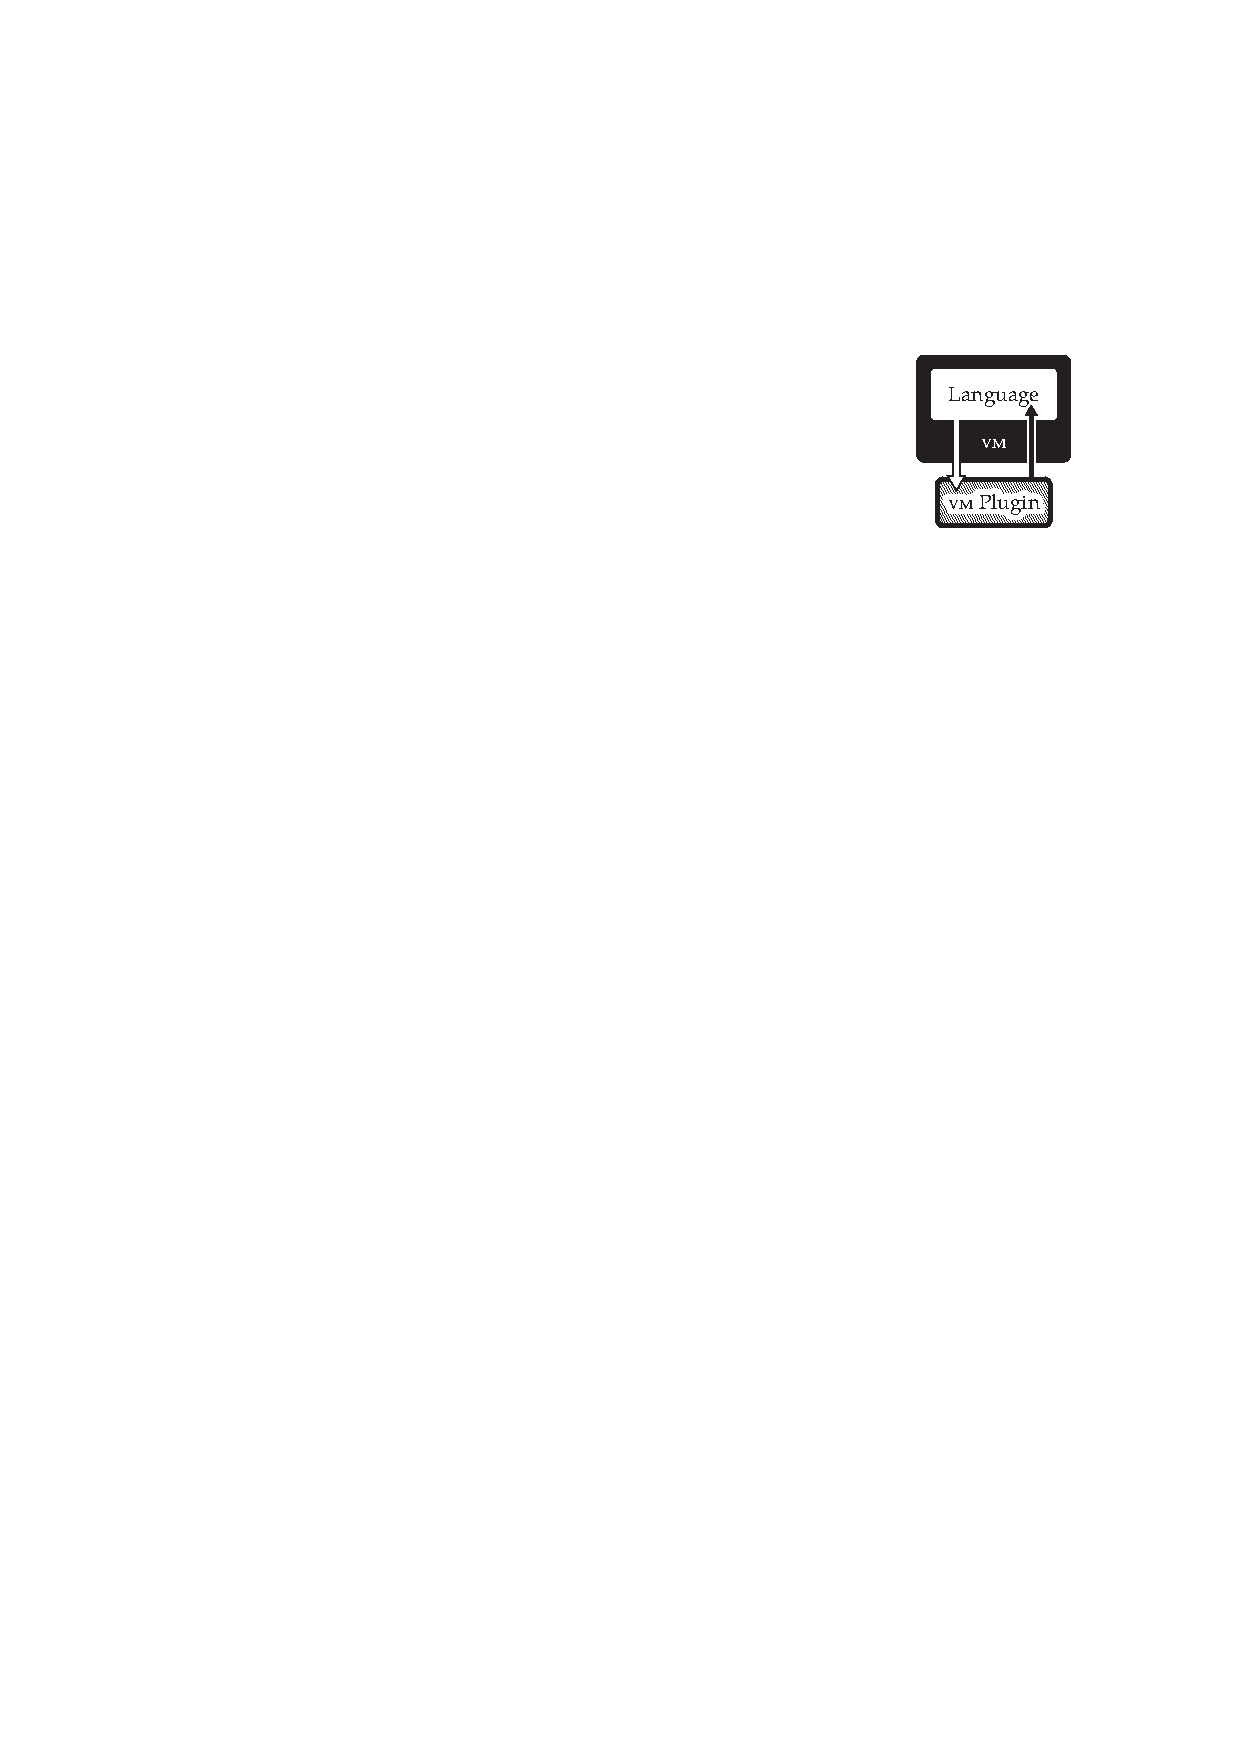
\includegraphics[scale=\imagescale]{extension-plugin}
		\caption{Language using features from a separate \VM plugin.}
	\end{subfigure}
	
	\caption[Language Extension Mechanisms]{Comparison of different extension mechanisms}
	\figlabel{benzo-extensionComparison}
\end{figure}

%----------------------------------------------------------------------------
\subsection{Language-side Library}
%----------------------------------------------------------------------------

The most straight forward solution for extending a language is to write libraries within the language itself. 
This option provides the advantage that the aggregate behavior is accessible and evolvable for any language developer.
However, language-side libraries are constrained by the underlying managed language runtime.
The \VM separates the language from the low-level internal details.
As a consequence language-side libraries are not feasible for all feature requirements.
For instance the previously mentioned example of instrumenting the language runtime is not possible as a standard language-side extension without a considerable performance loss.
So, even though we prefer extensions and optimizations at language-side, there are certain limitations of a managed language runtime that can not be circumvented.
If all language-side optimization opportunities have been exhausted it is exposing the need to resort to lower level approaches.

\begin{quote}
Language-side libraries are constrained to the capabilities of the underlying \VM and thus not general enough. 
Additionally not all performance bottlenecks can be addressed at language-side.
\end{quote}

%----------------------------------------------------------------------------
\subsection{Language-side Reflective Extensions}
%----------------------------------------------------------------------------

This is a specialization of the previous approach but in the context of reflective environments.
For instance, Meta Object Protocols (\MOP) \cite{Kicz91a} based on reflection \cite{Maes87a} are used to define certain control points in the system to change the language.
By composing meta objects it is possible to even modify the semantics of the language. 
Several languages such as \PH, \ST, \urlfootnote{\Python}{http://python.org/}, \urlfootnote{Ruby}{http://www.ruby-lang.org/}, and others provide reflective capabilities with different depths \cite{Ande98a,Van10a}.
However, most modern programming languages only have very limited support for intercession.
Hence the possibilities for dynamically changing language semantics or features are limited. 
Furthermore reflective capabilities are hard to implement efficiently.
Reflection imposes substantial performance penalties on most computations by postponing bindings \cite{Male96a}. 
Nevertheless, there are exceptions for a subset of reflective behavior which are implemented efficiently using a high-level MOP \cite{Vran12a}.
Though these approaches remain as a few exceptions.
In the typical low-level \VM it is difficult to gain reflective access to language-side objects.
Similar to the previous case, our goal is to extend language features in a general way and it was shown that this is only partially possible by reflective extensions. 

\begin{quote}
Reflective capabilities are not enough for general extensions. Even when suitable, they usually pose a significant performance overhead up to the point where they become unfeasible.
\end{quote}

%----------------------------------------------------------------------------
\subsection{\VM Extensions / Plugins}
\seclabel{benzo-vm-extensions}
%----------------------------------------------------------------------------
\sm{Yes, I think all that needs to be folded into chapter 2}
Another approach to extend add new features to a programming language is to extend the \VM.
At this level we differentiate between two extension mechanisms: \VM plugins and modified \VMs itself.
Plugins are direct bindings to external libraries described at \VM-side or libraries linked to the \VM executable \cite[Ch.\ 5]{Blac09a}. 
They provide a performance boost in comparison to pure language-side solutions.
Using highly optimized native libraries it is straightforward to outperform code written at language-side.
Typically, even very complex \VMs such as the \Self \VM \cite{Unga07a} provide a clean interface to write plugins.
Missing high-level concepts make them harder to maintain than language-side code.
Depending on the added feature the plugin interface may prove to be too inflexible and the only choice is an modified \VM.
Such a fork comes at an even higher cost of maintenance.
In the following paragraph we will explain the these two main limitations we found when working with plugins: a certain abstraction mismatch compared to host language and the limitations imposed by a clean plugin interface.


\subsubsection*{Problem: Abstraction Mismatch}
Plugins are commonly written in the same language as the \VM, at a low abstraction level.
The abstraction difference compared to a language-side extensions makes it difficult for standard programmers to modify or write \VM plugins.
Few exceptions are self-hosted languages \cite{Unga05a,Wimm13a,Rigo06a}.
To support a fluent development process, \VMs should come with an infrastructure for building extensions at same abstraction level as the provided language.
Instead \VMs tend to be rather complex which includes the whole development cycle.
For example, only a few \VMs have high-level debugging facilities \cite{Inga97a,Unga05a,Wimm13a}.
It is more common to be stuck in the compilation step waiting for the debugging binary to be ready.

\paragraph{\VM Generation Framworks}
The lack of abstraction for \VM-level extensions can is addressed by \VM generation frameworks in general.
They try to abstract away the complexity of the \VM and use high-level languages as compiler infrastructure.
A very successful research project is \urlfootnote{\textsc{Jikes} Research \VM}{http://jikesrvm.org/} (former \textsc{Jalapeño})~\cite{Alpe99a}.
It uses \Java to metacircularly define a \Java environment which then generates the final \VM.
A similar framework is \urlfootnote{\PyPy}{http://pypy.org/} \cite{Rigo06a} a \VM framework including an efficient \JIT. 
\PyPy uses a restricted subset of the  \textsc{Python} language named \textsc{RPython} which is then translated to various low-level backends such as C or \textsc{llvm} code.
There exist several different high-level language \VM implementations on top of \PyPy such as \ST \cite{Bolz08a} or \textsc{Prolog}.
However, its main focus lies on an efficient \JIT generator mainly for a \Python interpreter, and not on a direct, language-side assembler interface.
\PyPy encourages to use reflection at compile-time which helps to write a maintainable code base.

\subsubsection*{Problem: Plugin Limitations}
Once a programmer is fluent at \VM-level a clean plugin interface is a big aid in terms of maintenance.
However, certain functionality can not be added by simply creating a separate plugin that encapsulates the new feature.
Prominent examples are \JIT support, immutability or first-class handles \cite{Arna13a}.
In all these examples core pieces of the \VM have to be modified: the \VM has to be forked.
From a \VM maintenance point of view, forks have to be avoided if possible and should only be used for critical performance issues that can not be properly addressed at language-side or with plugins.

From our experience with \PH, even promising \VM experiments are not maintained for a long time.
An example for that is the modified \VM supporting back-in-time debugging implemented for an early version of \PH and \Squeak \cite{Lien08b}.
The features would improve debugging without a doubt.
However, the \VM evolved in the mean time adding new features required by newer versions of \PH.
As a result the back-in-time enabled \VM is no longer compatible with \PH.
Presumably it would be easier to port the back-in-time debugger to a new \PH version if it were implemented purely at language-side.


\paragraph{High-level Low-level Programming}
High-level low-level programming \cite{Fram09a} encourage to use high-level languages for system programming.
Frampton et al. present a low-level framework packaged as \textsc{org.vmmagic}, which is used as system interface for \Jikes, an experimental \Java \VM.
Additionally their framework is successfully used in \textsc{mmtk} \cite{Blac04a} which is used independently in several other projects.
The \textsc{org.vmmagic} package is much more elaborate than \B but it is tailored towards \Java with static types.
Methods have to be annotated to use low-level functionality.
Additionally the strong separation between low-level code and language-side application does not allow for reflective extensions of the language runtime.
Finally, they do not support the execution nor generation of custom assembly code in the fly.


\begin{quote}
VM extensions provide good performance at the cost of maintainability. 
Moreover this approach implies resorting to pure low-level development where tools and abstraction advantages from high-level languages are restricted.
\end{quote}

%----------------------------------------------------------------------------
\subsection{Hybrid Extensions}
%----------------------------------------------------------------------------

The last approach is to reuse an existing library usually implemented in a foreign language.
The languages interact through a well-defined Foreign Function Interface (\FFI).
\FFI-based extensions are a hybrid approach between pure language-side extensions and \VM-side ones.
Interaction with native libraries is supported by a dedicated \VM functionality for calling external functions.
This allows for a smooth interaction of external code and language-side code.
\FFI-based extensions share the benefits of a maintainable and efficient lan\-guage-side library with modest implementation efforts.
However, \FFI is only a bridge or interface for allowing the interaction of different languages. 
It is not possible to directly synthesize new native features from language-side.
For this purpose we have to interact with a custom-made native library.
From an extension point of view this is close to the \VM extensions discussed previously.

Additionally to the interface limitations, there exists a performance overhead in \FFI for making the interaction between different languages possible. 
This is due to marshalling arguments and types between both languages \cite{Fish00a,Repp06b}.


Other high-level languages such as \Lua leverage \FFI performance by using a close interaction with the \JIT.
\textsc{Luaffi}\footnote{\url{https://github.com/jmckaskill/luaffi/}} for instance is an efficient \Lua implementation that inlines \FFI calls directly into the \JIT compiled code.
Similar to \B this allows us to minimize the constant overhead by generating custom-made native code.
\Luajit is mainly written in C which has clearly different semantics than \Lua itself.
Compared to our approach the efficient \VM implementation suffers from the shortcomings described in \secref{benzo-vm-extensions}. 

Kell and Irwin \cite{Kell11a} take a different look at interacting with external libraries.
They advocate a \Python \VM that allows for dynamically shared objects with external libraries.
It uses the low-level \textsc{Dwarf} debugging information present in the external libraries to gather enough metadata to automatically generate \FFIs.
However, they do not focus on the reflective interaction with low-level code and the resulting benefits. 

\textsc{Quicktalk} \cite{Ball86a} follows a similar approach as the dynamic primitives in \WF.
However, Ballard et al. focus mostly on the development of a complex compiler for a new \ST dialect.
Using type annotations \textsc{Quicktalk} allows for statically typing methods.
By inlining methods and eliminating the bytecode dispatch overhead by generating native code \textsc{Quicktalk} outperforms interpreted bytecode methods.
Compared to \WF \textsc{Quicktalk} does not allow to leave the language-side environment and interact closely with the \VM.
Hence it is not possible to use \textsc{Quicktalk} to modify essential primitives.

A notable exception to the metacircular \VMs mentioned earlier is the \Self implementation \textsc{Klein} \cite{Unga05a}.
Unlike typical other metacircular approaches it does not strictly separate compile-time and runtime.
The reified \VM concepts are available at runtime, which is a result from implementing the typical \VM pieces at language-side.
Compared to our approach, \textsc{Klein}'s bridging efforts are much more complete.
However, \textsc{Klein} is built on a completely new \VM infrastructure, whereas \B requires only few changes to achieve its functionality.

\begin{quote}
Hybrid extension are the most promising.
They allow for a seamless interaction from high-level language-side to low-level functionality.
However, most existing solutions target only specific use cases and can not be reused for other applications.
\end{quote}


% ===========================================================================
\section{Limitations of Benzo}
\seclabel{benzo-problems}
% ===========================================================================
In this section we will point out the current limitations of the \B framework.
As we outlined in \secref{benzo-performance} \B is a promising alternative to building \VM-plugins.
Our prototype use cases, the dynamic primitives and the language-side \JIT compiler, even suggest that \B can be used as a replacement for certain \VM-level modifications.
However, throughout the development of these tools we also noticed certain drawbacks and limitations of the current \B implementation.
We will now discuss the following three main issues in more detail: robustness, debuggability and portability.
\sm{Be specific: for example...

You are making a claim here, you want that one to be verifiable and precise}

% -----------------------------------------------------------------------------
\subsection{Robustness}
\seclabel{benzo-problems-robustness}
% -----------------------------------------------------------------------------

The first immediately visible flaw of \B is that there is currently no support for running the native code in a protected environment.
\B directly transfer the execution context to the generated native code without protection.
Whilst this makes sense from a performance point of view for a stable piece of native code, it is nuisance during development.
The most common errors we noticed during development were cause due to stack misalignment and access to invalid memory region.
The latter one is also typical for C development, whereas creating a misaligned stack in pure C is not possible.

\begin{stcode}[caption={Simple \B code possibly leading to an unbalanced stack.}]{}
Benzo x86 generate: [ :asm |
	asm push: asm EAX ]
\end{stcode}

\begin{stcode}[caption={\B code possibly leading memory access violation.}]{}
Benzo x86 generate: [ :asm |
	asm mov: asm EAX ptr to: asm EAX ]
\end{stcode}

\noindent In \PH it is possible to willingly corrupt the stack by for instance injecting a wrong sender as illustrated with following the code example.
%
\begin{stcode}[label=lst:benzo-pharo-stack-corruption]{}
thisContext instVarNamed: #closureOrNil put: 1.
\end{stcode}
%
However, it is not very common to directly modify the current context in \PH and it requires rather deep knowledge of the system to break the stack explicitly.
\sm{Really? You showed me in one line how to do it}

In \B the standard developer will most probably be more familiar with \PH than with C or even Assembler, which will easily lead to the aforementioned errors.
\sm{So, it is not the right tool for the job, because it is too low level?

I would just leave out the 'standard developer', even experts make mistakes}
Which means that we have to be prepared for these common errors.
Currently the active operating system process will be killed when the misaligned stack eventually lead to an invalid memory access.
From a \PH point of view this is unacceptable behavior.
Typically every error is revealed in \PH by opening a debugger, giving the programmer a chance to figure out the problem at hand.
Enabling debugging support for the low-level \B code is not that easy as we will show in the following \secref{benzo-problems-debugging}.

As a first step we should provide a debug mode for \B where the low-level errors do not terminate the main process.
The most simple way to achieve this is by forking the whole \VM process at the moment the native \B code is activated.
However, the current implementation of the \PH \VM does not support clean forking, even so close implementations such as \Squeak supports forking with a specific \urlfootnote{\VM plugin}{http://wiki.squeak.org/squeak/708/}.
Implementing a debugging version of the \B plugin to activate native code in a forked process would solve this issue, though at the cost of an additional primitive.
\sm{Why can't you do it in benzo?}

Addressing faulty stack management requires more effort.
One possibility is to use an existing \ASM simulation framework and run the code in there and check for unbalanced stack operations.
This difficulty leads us the second issue with \B.

% -----------------------------------------------------------------------------
\subsection{Low-level Debugging}
\seclabel{benzo-problems-debugging}
% -----------------------------------------------------------------------------
The second main limitation of \B is the lack of a dedicated debugger.
\PH inherits the long standing tradition of \ST to provide an excellent debug interaction for programmers.
\sm{What is with the bochs plugin? That should provide you with everything you need to make debugging native code }

The \PH debugger shows the stack, the current receiver along with the temporary variables and argument.
However when working with \B this important tool is no longer available.
Currently the only way to debug \B code is to launch the \VM upfront in a C debugger such as \GDB or \LLDB.
However, the debug interaction is rather limited compared to \PH.
Not only does the programmer have to resort to an external tool, but there are only a handful mostly proprietary standalone debuggers available.

For a better low-level debugging experience we have to rely on a complete \textsc{ide} such as \textsc{Eclipse} or \textsc{Xcode}, a rather cumbersome overhead to standard \PH programming.
\sm{Cut all the Pharo related assessment, just discuss that you want to debug on the same high level you are programming in and give examples of functionality you desire. Pharo is not essential here}

Besides using these external tools there is no simple alternative.
The only way to provide a seamless debugger is to either build on the fork solution presented in the previous \secref{benzo-problems-robustness} or a separate simulator.
System libraries such as \ptrace enable debugging for an external process.
It would be possible to write bindings to this library with an \FFI from within \PH and debug a \B-enabled method this way.

Even so this would be a great step forward compared to the current infrastructure it implies that the programmer anticipates debugging.
Something that is very uncommon in \PH as the debugger is tightly integrated into the standard development environment.
A potential solution to this problem would be to install low-level signal handlers which try to backtrack from signals triggered by memory access violations such as \ttt{SIGBUS} and \ttt{SIGSEGV} under Linux.
\sm{Pfff, again, your writing style makes that look like an undesirable afterthought, no, use the OS to do the right thing. That's exactly what you want to do.

And present it like that: here, a sketch for a possible solution. Complete debugging support is outside the scope for this thesis, but if you want, that's how you could continue our work...}

\begin{figure}[h]
	\centering
	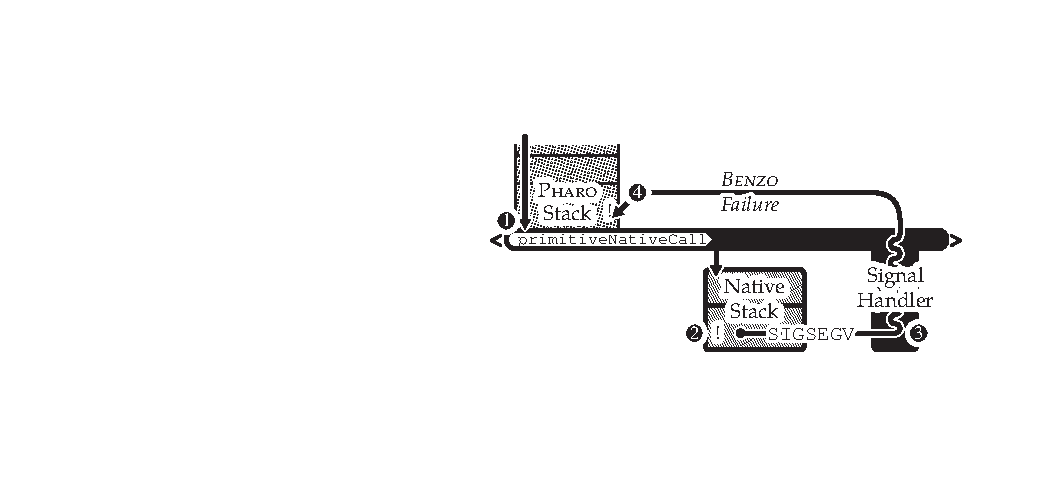
\includegraphics[scale=\imagescale]{benzo-debugger}
	\caption{\B Debugger Outline}
	\figlabel{benzo-debugger}
\end{figure}

The following list explains the detailed steps of \figref{benzo-debugger}.
\todo{missing link from the text}
\begin{enumerate}
	\item Standard \PH method activating a \B-enabled method through the \ttt{primitiveNativeCall} primitive.
	\item Native code causing a memory access violation (for example \ttt{SIGSEV}) which can not be handled by \PH directly.
	\item Low-level signal handler is activated by the operating system and tries to walk back the native stack up to the \ttt{primitiveNativeCall} activation.
	\item After successfully finding the \ttt{primitiveNativeCall} the signal handler sends a \B failure back to \PH.
\end{enumerate}

\noindent We assume that with the outlined mechanism an important fraction of the occurring memory access violations could be handled adequately in \PH.
However, since there is no real protection in the native code, there is no guarantee that the main \PH \VM can continue working.
Faulty native code might have corrupted the main \PH stack or heap beyond repair.
Nevertheless, this scheme could bring approximate a \PH like user experience for native \B code.
\sm{Instead of Pharo -> high level (again, this is one of your thesis goals, your thesis goal is not improving Pharo, but to contribute to the global set of knowledge)}


% -----------------------------------------------------------------------------
\subsection{Platform Independence}
\seclabel{benzo-problems-platform-independence}
% -----------------------------------------------------------------------------
The previous two issues discussed, robustness and debuggability, both target the integration into the existing \PH development environment.
This third issue on the other hand is related to the system integration: platform independence.

The \textsc{Intel x86} instruction set is widely distributed and supported by a variety of operating systems and thus the primary choice as native backend for \B.
Since the generated code is independent of C functions it works on all platforms with x86 support.
However, other architectures such as \ARM start to be more widespread and inevitable \B has to be ported on other platforms.
%A prominent example are \textsc{Apple}'s tablets and mobile phones running iOS.
In contrast to \PH itself, \B does not work on \ARM platform since all the low-level code is written in terms of x86 instructions.
While there is no way around a \ARM version of the underlying assembler, we think that porting all existing \B routines is too costly.
Instead we suggest to use an intermediate format that is platform independent more high-level than direct assembler instructions.
We call this intermediate format \VCPU and it has the following properties:
%
\begin{itemize}[noitemsep]
	\item High-level three-address-code (\TAC) instructions
	\item Automatic stack-management
\end{itemize}
%
Along with the ongoing work for this thesis we already started implementing \VCPU as a fork of the original compiler infrastructure of the \P \VM.
\sm{What is this? Why is that discussed here, and not integrated with the whole benzo story? If you got the design, and a more or less working solution sell it as key aspect!

That is eh solution you envision, in the limitations section you can then clarify that virtualcpu is buggy, or only partially implemented, so that you bypass it for many things...(well, if virtualcpu has sufficient maturity, but i }

\paragraph{\VCPU}
\seclabel{benzo-problems-vcpu}
In this following paragraph we are going to highlight the benefits and usage of \ugh{this intermediate format}.
\VCPU is based on a \TAC to simplify the adoption of optimizations such as \SSA.
These \TAC instructions take the following form:
%
\begin{stcode}{}
result := argument1 OP argument2
\end{stcode}
%
There are three operands involved, \ttt{result}, \ttt{argument1} and \ttt{argument2}, from which the name of this instruction format originates.
Based on this assumption, each standard \VCPU instruction returns a temporary variable which can be used for further operations.
The following code example outlines the basic usage of \VCPU:
%
\begin{stcode}[
	label={lst:benzo-problem-vcpu}, 
	caption={Basic \VCPU Example}
]{}
Benzo vcpu x86 generate: [ :asm | | temp1 temp2 |
	temp1 := asm memoryAt: 16r12345.
	temp2 := asm uint: 2.
	asm return: temp1 + temp1 ]
\end{stcode}
%
Which corresponds to the same functionality expressed in the following x86 instructions:
%
\begin{stcode}{}
Benzo x86 generate: [ :asm |
	asm mov: 16r12345 ptr to: asm EAX.
	asm add: asm EAX with: 2.
	asm return ]
\end{stcode}
%
To get to the final native instructions the \VCPU infrastructure compiles the high-level instructions to the specific backend.
The current compiler is divided into the following passes:
%
\begin{itemize}[noitemsep]
\item Platform Specific Transformation
\item Register Allocation
\item Superfluous Assignment Remover
\item Platform Specific Assembler
\end{itemize}
%
Applying these compiler passes to the example in \lstref{benzo-problem-vcpu} yields the following native instructions:
%
\begin{stcode}{}
mov   6 -> EDX
mov   2 -> ECX
add EDX,   ECX
mov ECX -> EAX
return 
\end{stcode}


\noindent With a properly parametrized register allocator and a separate constant folding pass the result could be greatly improved.
%A more detailed motivation and implementation details of this compiler are given in the following \secref{future-mate-compiler}.

% ===========================================================================
\section{Conclusion and Summary}
\seclabel{benzo-conclusion}
% ===========================================================================

In this chapter we presented \B, an integral approach for reflective high-level low-level programming.
\B consists of three core parts: \AsmJIT a language-side assembler, a set of primitives to activate native code and language-side library to handle dynamic code installation and activation.

\B promotes a smooth and powerful interaction with the low-level world by dynamically generating native code from language-side.
This enables to exploit the underlying platform capabilities when strongly needed without leaving the host development platform.
Most of the \B infrastructure is implemented at language-side and thus susceptible to modification. 
As a result, \B advocates the use of development tools and abstraction level of the high-level language for as much as possible or desired.

\paragraph{\B Applications}
Based on \B we outlined in this chapter three example applications: an \FFI in \secref{benzo-ffi}, dynamic primitives in \secref{benzo-waterfall} and a language-side \JIT compiler in \secref{benzo-nabujito}.
Typically all these applications require either a modified \VM or a dedicated plugin while our implementations are based on a central framework for low-level interaction.
In this chapter we only outlined these application to stress the fact that they use \B and only the following chapters will shed light on the implementation details of these three applications.

\paragraph{\B Performance}
Using the three \B-based applications we evaluate the performance of \B compare to a typical \VM-level implementation.
In summary we note that \B's code generation at language-side is slow compared to a single invocation the final native code.
However, this is only a one-time overhead since \B caches native code transparently at language-side.
Additionally we generate specific native code for each different application we easily outperform a static solution.
This becomes evident with the \FFI implementation that is based on \B.
Our mature \FFI implementation outperforms an existing C-\FFI implementation by a factor of 1.5 even though we control every aspect from language-side.

By combining high-level reflection capabilities with efficient low-level code we manage to do dynamic primitive instrumentation and reuse the code for primitive operations which is duplicated on the standard \JIT approach.
We also show that since our \JIT compiler poses only a one-time overhead when generating native code. 

\paragraph{\B's Limitiations}
Even though \B allows us to implement the three example applications at language-side, the complete development interaction requires improvement.
Currently there is not protection against faulty assembler code nor support for a low-level debugger.
To clearly support the theory of boundary-less low-level interaction a basic debugging infrastructure is required as outlined in \secref{benzo-problems}.

\paragraph{\B Outlook}
\B shows that promoting clear interfaces for controlling low-level code completely from language-side produces efficient solutions for system programming without resorting to pure low-level solutions.
Our set of \B-based applications shows that it our approach is feasible and efficient.
At the first sight \B is a simple application to invoke native code but we think that it opens doors for a new kind of language runtime.
In this envisioned system there is no longer a clear barrier between \VM and language-side.
This might seem far fetched but becomes more apparent when having a look at the \JIT of \PH which reimplements a performance critical set of primitives in its own native code.
Essentially this is code duplication since the primitives already exist as normal C code in the \VM sources.
With \B and the described dynamic primitives we should reuse the same code base for creating the \JIT representation of the primitive.\\

\noindent After presenting the basis of our high-level low-level programming framework in \PH we will focus on its application in the following chapters.


% =============================================================================
\ifx\wholebook\relax\else
    \end{document}
\fi